%%%%%%%%%%%%%%%%%%%%%%%%%%%%%%%%%
%%%%%%%%Dokumentdefinition%%%%%%%
%%%%%%%%%%%%%%%%%%%%%%%%%%%%%%%%%
\documentclass[oneside,11pt,a4paper,numbers=noenddot]{scrreprt} 
\usepackage{geometry}
\geometry{a4paper, top=25mm, left=30mm, right=25mm, bottom=20mm, headsep=5mm, footskip=12mm}

%%%%%%%%%%%%%%%%%%%%%%%%%%%%%%%%%%%%%%%%%%%%%%%%%%%
%Inputfile für Packages (hält das Dokument sauber)%
%%%%%%%%%%%%%%%%%%%%%%%%%%%%%%%%%%%%%%%%%%%%%%%%%%%
%%%%%%%%%%%%%%%%%%%%%%%%%%%%%%%
%Kopf- und Fußzeilendefinition%
%%%%%%%%%%%%%%%%%%%%%%%%%%%%%%%
\usepackage[headsepline,footsepline]{scrlayer-scrpage}	%mit Trennlinien
\pagestyle{scrheadings}					%Seitenstil umdefiniert
\clearpairofpagestyles					%Definition leermachen
\renewcommand{\chapterpagestyle}{scrheadings}		%Kapitelseitenstil umdefiniert
\renewcommand{\chaptermark}[1]{\markboth{\ #1}{}}	%Definition Kapitel?berschrift=\leftmark
\ohead{\leftmark}				%äußere Kopfzeile
\chead{}						%mittlere Kopfzeile
\ihead{}						%innere Kopfzeile
\ofoot{\thepage}				%äußere Fu?zeile
\cfoot{}						%mittlere Fu?zeile
\ifoot{}						%innere Fu?zeile

%%%%%%%%%%%%%%%%%%%%%%%%%%%%%%%%%%%%%%%
%%%%%%%deutsche Zeichenkodierung%%%%%%%
%%%%%%%%%%%%%%%%%%%%%%%%%%%%%%%%%%%%%%%
\usepackage[utf8]{inputenc}
\usepackage[english,ngerman]{babel} 

%%%%%%%%%%%%%%%%%%%%%%%%%%%%%%%%%%%%%%%%%%%%%%
%%%%%%%%%%%%Verschiedene Schriftarten%%%%%%%%%
%%%%%%%%%%%%%%%%%%%%%%%%%%%%%%%%%%%%%%%%%%%%%%
%\usepackage{crimson}
%\usepackage[adobe-utopia]{mathdesign}
%\usepackage{libertine}
%\usepackage{lmodern}
%\usepackage{kpfonts}
\usepackage{stix}
%\usepackage{libertinust1math}
\usepackage[T1]{fontenc}
%\renewcommand*\familydefault{\sfdefault}

%%%%%%%%%%%%%%%%%%%%%%%%%%%%%%%%%%%%%%%%%%%%%%
%%%%%%%%%%%%%%%Zusatzpackages%%%%%%%%%%%%%%%%%
%%%%%%%%%%%%%%%%%%%%%%%%%%%%%%%%%%%%%%%%%%%%%%
\usepackage{a4wide}
\usepackage{longtable}
\usepackage{longtable}
\usepackage[locale=DE]{siunitx}
\usepackage{eurosym}					%Fancy ? Zeichen
\usepackage{acronym}					%Abk?rzungsverzeichnis
\usepackage{wasysym}					%Symbole und Sonderzeichen
\usepackage{longtable}					%Formelzeichentabelle/lange Tabelle
\usepackage{romannum}					%R?mische Zahlen
\usepackage{wrapfig}					%Bilder nebeneinander/ Text neben Bild
\usepackage{floatflt,epsfig} 				%Bilder im eps-format einf?gen
\usepackage{exceltex}					%Exceldokumente einbinden
\usepackage{multirow}					%Tabellenzellen verbinden
\usepackage{multicol}					%Mehrere Spalten
\usepackage{graphicx}					%fuer bilder
\graphicspath{ {./bilder/} }

\usepackage{chngcntr}
\counterwithout{figure}{chapter}

\usepackage[hyphens]{url}				%Websites einbinden
\usepackage{hyphsubst}
\usepackage{pdfpages} 					%direkt pdf Datein einbinden
\usepackage{amsmath}					%matheumgebung f?r Formeln und Gleichungen
\usepackage{booktabs}					%ich glaube f?r links im PDF
\usepackage{capt-of}					%Captions f?r non-float-Objekte
\usepackage{appendix}					%erm?glicht das erstellen von Anhangsverzeichnissen
\usepackage{tikz}					%tikz Paket f?r Grafiken + Definitionen
\usepackage{multicol}               % Mehrspaltige Bereiche	
\usepackage[euler]{textgreek}		%greek chars without math mode
\usepackage{caption}				%multiline caption
\usepackage{tabularx}
\usetikzlibrary{arrows,positioning}
\usetikzlibrary{decorations.pathmorphing}
\usetikzlibrary{shapes.geometric}



%%%%%%%%%%%%%%%%%%%%%%%%%%%%%%%%%%%%%%%%%
%%%%%%%%%%%%%%special Stuff%%%%%%%%%%%%%%
%%%%%%%%%%%%%%%%%%%%%%%%%%%%%%%%%%%%%%%%%
\usepackage[colorlinks,    				%PDF linked Verzeichnis
pdfpagelabels,
pdfstartview = FitH,
bookmarksopen = true,
bookmarksnumbered = true,
linkcolor = black,
plainpages = false,
hypertexnames = false,
citecolor = black,
breaklinks = true,
allcolors = black] {hyperref}  

\usepackage[english,ngerman]{cleveref} 				%Bessere Referenzen nach hyperref!

%\renewcommand{\labelitemi}{-}   %aufzählungszeichen strich statt punkt - beliebig anpassbar
\usepackage{csquotes}
\usepackage[backend=biber,
			sorting=none
			]{biblatex}
\addbibresource{literature.bib}

	

\sloppy 						%"schlampiger" Blocksatz
\parindent0cm 					%Absatzeinzug

\usepackage{setspace} 			%Zeilenabstand
\onehalfspacing
%\singlespacing
%\doublespacing

%%%%%%%%%%%%%%%%%%%%%%%%%%%%%%%%%%%%%%%
%hier startet das eigentliche Dokument%
%%%%%%%%%%%%%%%%%%%%%%%%%%%%%%%%%%%%%%%
\begin{document}				
	\pagenumbering{Roman}				%Seitennummerierung auf römisch geändert
	\begin{titlepage}					%gesondert formatierte Titelseite
		
%% Document properties %%%%%%%%%%%%%%%%%%%%%%%%%%%%%%%%%%%%%%%%%%%%%%%%
\newcommand{\projname}{Der Projektname}
\newcommand{\titel}{Seminararbeit}
\newcommand{\authorname}{Michael Smirnov}
\newcommand{\thesisname}{Medieninformatik}
\newcommand{\untertitel}{Mobile App Development Frameworks}
\newcommand{\Datum}{06. Juli 2021}


\titlehead{
  \centering
  
\includegraphics[width=.5\textwidth]{bilder/fhw}\\
  \bigskip
  \textsc{\Large Department of Computer Science}
}

\subject{\thesisname}
\title{\titel}
\subtitle{\Large \untertitel}
\date{\vspace{-1cm}{\small Eingereicht am:}\\\medskip\Datum}
\author{}
\publishers{\vfill
  \normalsize

  

    {\small Eingereicht von:} \\
    \smallskip
  	{\Large \authorname}\\
     Windfeld 37\\
     22559 Hamburg\\
     Tel.: 0176~40022200\\
     E-Mail: minf103430@fh-wedel.de\\

    

    \bigskip
       


      {\small Betreuer:}\\
      \smallskip
      {\Large Prof. Dr. Andreas Häuslein}\\
      Fachhochschule Wedel\\
      Feldstraße 143\\
      22880 Wedel\\
      Tel.: (041\,03)~80\,48-42\\
      E-Mail: hs@fh-wedel.de\\
         

}


\maketitle 		
	\end{titlepage}
	\thispagestyle{empty}
	\cleardoublepage
		
	
	%%%%%%%%%%%%%%%%%%%%%%%%%%%%%%%%%%%%%%%%%%%%%%%%%%%%%%%%%%%%%%%%%%%%%%
	%\input{kapitel/01_Notwendiges.tex}%Vorwort, Editorial, Erklärungen, Vermerke%%
	%%%%%%%%%%%%%%%%%%%%%%%%%%%%%%%%%%%%%%%%%%%%%%%%%%%%%%%%%%%%%%%%%%%%%%
	
	
	\newpage
	%\begin{singlespace}
	
	%%%%%%%%%%%%%%%%%%%%%%%%%%%%%%%%%%%%%%%%%%%
	%%%%%%%%%%%%%%%Verzeichnisse%%%%%%%%%%%%%%%
	%%%%%%%%%%%%%%%%%%%%%%%%%%%%%%%%%%%%%%%%%%%
	\setcounter{secnumdepth}{2} 	%countertiefe für Verzeichnisse
	\setcounter{tocdepth}{2}		%Auflistungstiefe für Verzeichnisse
	\chaptermark{Inhaltsverzeichnis}
	\tableofcontents 						%Befehl für Inhaltsverzeichnis
	\newpage
	\listoffigures 							%Befehl für Abbildungsverzeichnis
	\addcontentsline{toc}{chapter}{Abbildungsverzeichnis} 		
	\chaptermark{Abbildungsverzeichnis}
	\newpage
	
	\listoftables							%Befehl für Tabellenverzeichnis
	\addcontentsline{lot}{chapter}{Tabellenverzeichnis}
	\chaptermark{Tabellenverzeichnis}
	\newpage
	
	\chapter*{Abkürzungsverzeichnis}
	\begin{acronym}
		\acro{SDK}{Software Development Kit}
		\acro{API}{Application Programming Interface}
		\acro{HTML}{Hypertext Markup Language}
		\acro{CSS}{Cascading Style Sheets}
		\acro{SASS}{Syntactically Awesome Stylesheets}
		\acro{HTTPS}{Hypertext Transfer Protocol Secure}
		\acro{PWA}{Progressive Web App}
		\acro{UI}{User Interface}
		\acro{UX}{User Experience}
		\acro{URL}{Uniform Resource Locator}
		\acro{JIT}{Just in Time}
		\acro{AOT}{Ahead of Time}
		\acro{DOM}{Document Object Model}
		\acro{VM}{Virtual Machine}
	\end{acronym}
	\addcontentsline{toc}{chapter}{Abkürzungsverzeichnis}		%ins Inhaltsverzeichnis schreiben
	\chaptermark{Abkürzungsverzeichnis}
	
	
	
	
	%\end{singlespace}
	\cleardoublepage
	\pagenumbering{arabic}			%ab hier arabische Seitenzahlen
	
	%Vorlagenkapitel
	\chapter{Einleitung}

Weltweit wurden im Jahr 2019 1.540.655 Smartphones verkauft. Diese Anzahl an verkauften Endgeräten folgt einem seit 2016 stabilen Trend von c.a. 1.500.000 vertriebenen Exemplaren jährlich. Aufgrund der weltweiten Covid-19 Pandemie sank die Anzahl an abgesetzten Smartphones global um 10.5\% auf 1.378.719 Einheiten, jedoch wird für das Jahr 2021 prognostiziert, dass sich der Markt erholt\cite{statista2_sales}\cite{gartner_sales}. In relativen Zahlen bedeutet dies, dass derzeit etwa 48\% der Weltbevölkerung ein Smartphone besitzen. Im Verglich dazu betrug der Anteil der Smartphonebesitzer im Jahr 2016 33,5\%\cite{bankmycell}.\\

Daraus ergibt sich, dass Smartphones sich hoher Beliebtheit erfreuen und inzwischen fest in unser alltägliches Leben integriert sind. Dies kann damit begründet werden, dass die Möglichkeit besteht eine Vielzahl verschiedener Apps zu installieren mit deren Hilfe das Gerät um eine Vielfalt an Funktionalitäten erweitert wird, die den Bedürfnissen und Wünschen des Nutzers entsprechen. Die verschiedenen Smartphones nutzen unterschiedliche Betriebssysteme, sodass eine App für die breite Masse mit den verschiedenen Plattformen kompatibel sein sollte, um eine möglichst große Anzahl an Nutzern zu erreichen.\\

Android und iOS stellen 99\% des Marktanteils der mobilen Betriebssysteme dar. Dabei ist Googles Android der Marktführer mit 72\% weltweit und iOS, Apples proprietäres Betriebssystem, mit ca. 27\% auf dem zweiten Platz \cite{stat1}. Somit stellen beide Betriebssysteme eine hinreichend große Verteilung dar, um im Folgenden berücksichtigt zu werden.\\

Bei Betrachtung der Relevanz von Betriebssystemversionen, fällt auf, dass Android Version 8 und höher auf 82\% aller Geräte zum Einsatz kommt. Im iOS Ökosystem ist die älteste relevante Version iOS 12.4 mit c.a. 7\% Anteil\cite{stat3}\cite{stat4}.\\

\newpage

Die Verteilung der Betriebssysteme und deren verwendete Versionen spielen bei der Evaluation des Entwicklungssatzes eine wichtige Rolle. Aufgrund der Tatsache, dass nicht alle Nutzer sofort das Betriebssystem aktualisieren, entsteht die Notwendigkeit eine mobile App auf den am meisten verwendeten Betriebssystemversionen explizit zu testen. Zudem müssen teilweise mehrere Versionen derselben App gepflegt werden, um ein breites Spektrum der Betriebssystemversionen zu unterstützen. Dieser Support verbraucht wertvolle Entwicklerressourcen, sodass eine Abwägung der relevanten Versionen notwendig wird\cite{flutter_support}. Ebenfalls relevant für einige Entwicklungsansätze sind die verschiedenen Web-Browser wie Firefox, Chrome oder Safari und deren Versionen. Auf die Eigenschaften und Unterschiede der verschiedenen Web-Browser wird jedoch im Laufe dieser Arbeit nicht näher eingegangen, da diese vor allem bei webbasierten Entwicklungsansätzen relevant sind, welche nur einen Teil dieser Seminararbeit ausmachen.\\

Ziel dieses Seminars ist es einen konzeptionellen Überblick über die derzeit vorherrschenden Mobile App Framework Technologien zu geben und auf die sich aktuell im Trend befindlichen näher einzugehen.
Es soll sowohl ein rudimentäres Verständnis über die verschiedenen Technologien als auch eine Basis geschaffen werden, auf welcher aufbauend Entscheidungen für oder gegen einen gewissen Ansatz getroffen werden können soll.\\


    \chapter{Theorie der \glqq Mobile App Development Frameworks\grqq}

\section{Definitionen}

\subsection{Mobiles Endgerät}

Im weiteren Verlauf wird der Begriff mobile oder mobiles Endgerät in Anlehnung an das National Institute of Standards and Technology (NIST) genutzt. Diese definieren ein mobiles Endgerät als ein kleines Datenverarbeitungsgerät, welches leicht von einer einzelnen Person getragen werden kann. Dieses Mobile Gerät ist darauf ausgelegt ohne physische Verbindung zu funktionieren. Es besitzt einen lokalen, nicht entfernbaren Datenspeicher und wird über einen längeren Zeitraum von einer verbauten Energiequelle betrieben. Mobile Geräte können auch Sprachkommunikationsfähigkeiten, eingebaute Sensoren, die es dem Gerät ermöglichen, Informationen zu erfassen (z.B. Fotografie, Videoaufnahme und Standortbestimmung) und/oder eingebaute Funktionen zur Synchronisierung lokaler Daten mit weiteren Standorten enthalten\cite{nist1}.

\subsection{App/Applikation}

Mobile Apps werden im Folgenden auch als App bezeichnet. Der Begriff App ist innerhalb kürzester Zeit in den Sprachgebrauch eingegangen und wird weithin als eigenständige Anwendung auf einem mobilen Endgerät verstanden.
Apps werden von eigenständig dafür ausgelegten Plattformen heruntergeladen, welche von dem Hersteller des Betriebssystems zur Verfügung gestellt werden, oder direkt aus dem Internet bezogen.
Beispiele dafür sind der App Store bei iOS-Systemen und der Google Play Store bei Android-Systemen\cite{heikGrundl}.
\newpage
\subsection{Software-Framework}

Der Begriff Mobile App Framework ist nicht einheitlich definiert und kann je nach Kontext auf eine andere Art und Weise verwendet werden. Im Folgenden wird der Begriff Framework folgendermaßen definiert: \\

Bei einem Software-Framework handelt es sich um eine Abstraktion von Details, welche notwendig wären, um ein bestimmtes Ziel zu erreichen. Ein Framework stellt dem Entwickler eine gewisse Grundfunktionalität zur Verfügung, auf welcher aufgebaut werden kann, um eigene Software zu schreiben. Grundbausteine von Frameworks sind abstrakte oder konkrete Klassen, welche beerbt erweitert oder direkt verwendet werden können.\\

Frameworks lassen sich anhand der Kontrolle des Programmablaufes von einer Library abgrenzen. Während Frameworks die Kontrolle über den Programmablauf behalten und an bestimmten Stellen den vom Anwendungsentwickler eingefügten Code ausführen, stellen Librarys eine Ansammlung von Funktionen dar, welche vom Code des Anwendungsentwicklers aus aufgerufen werden können. Jedoch ist der Übergang von Framework zu Library fließend und hängt auch stark von dem Kontext ab in welchem der Begriff verwendet wird.\\

Martin Fowler definiert den Unterschied folgendermaßen:

\blockcquote{fowler1}{
	\glqq Inversion of Control is a key part of what makes a framework different to a library. A library is essentially a set of functions that you can call, these days usually organized into classes. Each call does some work and returns control to the client.
	A framework embodies some abstract design, with more behavior  built in. In order to use it you need to insert your behavior into various places in the framework either by subclassing or by plugging in your own classes. The framework's code then calls your code at these points.\grqq
}

\begin{figure}[h]
	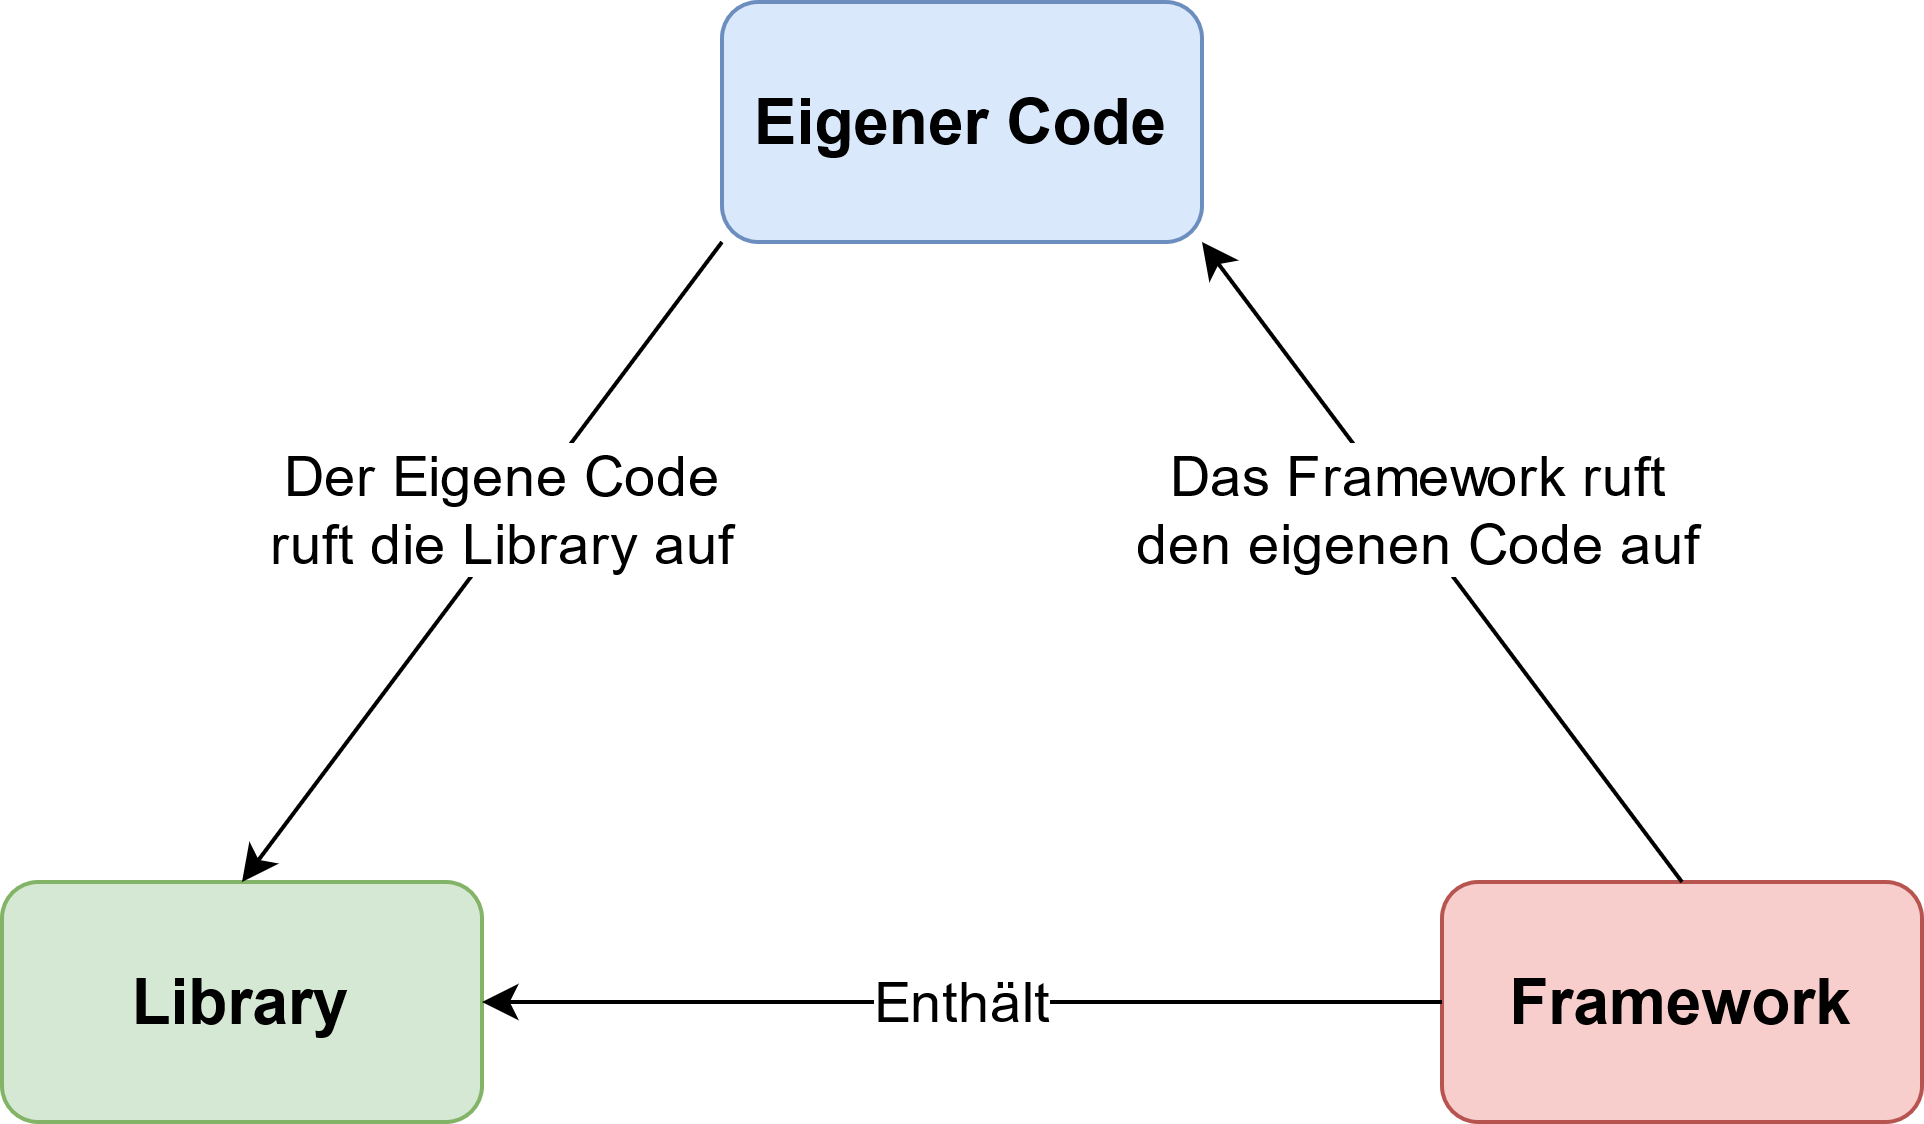
\includegraphics[scale=0.12]{frameworks}
	\centering
	\caption{Zusammenhang zwischen einer Library und einem Framework}
\end{figure}

\newpage

Zusätzlich zu der Unterscheidung zwischen Frameworks und Librarys existieren noch sogenannte \glqq opinionated\grqq\ und \glqq non-opinionated\grqq\ Frameworks bzw. Librarys. Bei opinionated Frameworks werden gewisse Vorgaben gemacht, z.B. wie die Ordnerstruktur des Projekts aussehen sollte oder wie gewisse Funktionen zu implementieren sind. Es wird ein Rahmen bereitgestellt, in welchem Beziehungen und Architektur der Komponenten vorgegeben werden. Abweichungen von diesem sind, je nachdem wie strikt diese durchgesetzt werden, schwer und nur mit viel Aufwand möglich. Non-opinionated Frameworks hingegen schreiben solch einen Rahmen nicht vor. Der Entwickler muss sich selber um bestimmte Aspekte wie z.B. den Anwendungszustand kümmern. Dies sorgt dafür, dass die Flexibilität auf Kosten der Komplexität erhöht wird\cite{opinionated}.\\

Ein Mobile Application Development Framework ist demnach ein Framework, welches die Struktur bereitstellt, eine Anwendung zu bauen, welche auf einem Mobilgerät ausgeführt werden soll.

\newpage
\section{Einsatzgebiete und Gründe für die Nutzung eines Mobile App Development Frameworks}

Die Gründe ein Framework in einem bestimmten Projekt zu nutzen sind sehr vielfältig und meist sehr individuell, da das Framework meist nur ein Hilfsmittel ist, um die Anforderungen an das Projekt zu erfüllen.\\

Bei Applikationen, dessen Zielgruppe Endbenutzer sind, besteht wie eingangs erwähnt die Notwendigkeit verschiedene Plattformen zu unterstützen, um eine größtmögliche Anzahl an Benutzern sicherzustellen. Dabei ist es finanziell und organisatorisch vorteilhaft nur eine einzige Codebasis pflegen zu müssen. Außerdem wird somit Feature, \ac{UX} und \ac{UI} Gleichheit sichergestellt.\cite{rieger_evaluation}\\

Die Herausforderung für mobile Endgeräte zu entwickeln, kommt nicht nur aus der Notwendigkeit für zwei unterschiedliche Plattformen mit verschiedenen Versionen zu entwickeln und diese über einen gewissen Zeitraum zu unterstützen, sondern auch durch die aufgesplitterte Android-Landschaft. Da Google Android als Betriebssystemplattform entwickelt, können Hersteller auf dieser aufbauend beliebige Modifikationen und Erweiterungen vornehmen\cite{andriod1}. Dies sorgt dafür, dass eine Vielzahl an unterschiedlichen Hard- und Softwarekombinationen existieren. Diese nutzen zwar alle Android als Plattform, das eigentliche Betriebssystem und die Hardware, auf der es läuft, unterscheiden sich trotzdem teilweise stark voneinander. 2015 gab es über 24.000 verschiedene Geräte, welche auf Android basierten von etwa 1.300 verschiedenen Herstellern\cite{opensignal1}.

\begin{figure}[h]
	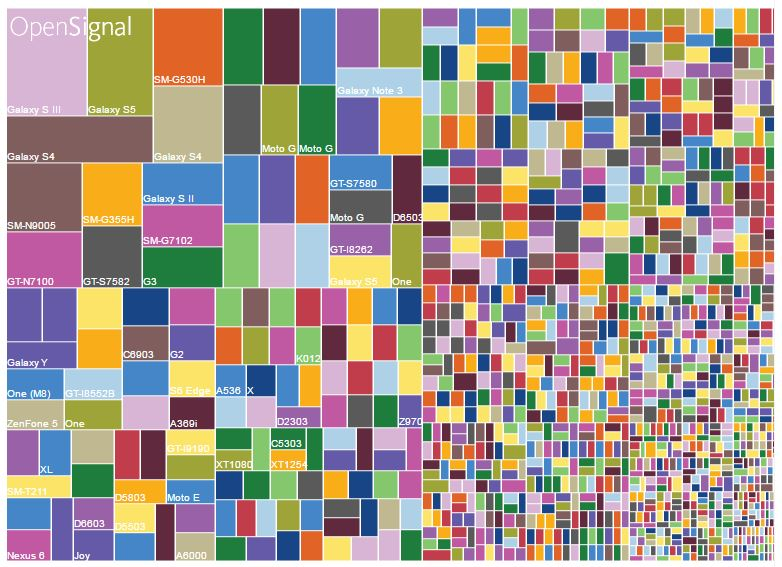
\includegraphics[scale=0.5]{androidfrag}
	\centering
	\caption[Visualisierung der Hardware-Fragmentierung von Android-Geräten]{Visualisierung der Hardware-Fragmentierung von Android-Geräten \cite{opensignal1}}
\end{figure}

\newpage
Hinzu kommt noch der Trend, dass immer mehr verschiedene Gerätetypen Android als Betriebssystem nutzen und dem User ebenfalls ermöglichen Apps auf diesen zu installieren. Zu den bereits bekannten Smartphones und Tablets sind in den letzten Jahren vermehrt Smartwatches, Autos und Smart TV Fernseher dazugekommen, welche ein Android-Basiertes Betriebssystem nutzen. Dies hat zur Folge, dass zusätzlich verschiedene Konnektivitätseigenschaften der Endgeräte berücksichtigt werden müssen. Zudem verschwimmen die Grenzen zwischen den Gerätetypen immer mehr. Jedes dieser verschiedenen Gerätetypen birgt Besonderheiten und Limitierungen, was die Entwicklung einer Anwendung, welche mit mehreren Typen kompatibel sein soll, teilweise stark verkomplizieren. Mit einigen der im Folgenden erwähnten Frameworks kann solch ein breites Spektrum an Endgeräten abgedeckt werden, jedoch wird im weiteren Verlauf der Arbeit näher darauf eingegangen, da diese Endgeräte teilweise der Definition von einem mobilen Endgerät nicht entsprechen und eine Berücksichtigung dieser den Rahmen sprengen würde.\\

Des Weiteren können Gründe für die Nutzung bestimmter Frameworks auch organisatorischer Natur sein und müssen nicht zwingend technisch begründet sein. Beispiele dafür können die Erfahrung und Größe des Entwicklungsteams, die Größe des Projekts, Vorgaben der Organisation, Lizenzen, verfügbares Budget und noch viele Weitere sein. Generell wird eine immer kürzere und effizientere Entwicklung von Software angestrebt, was eine Reduzierung von Entwicklungszeit und somit Kosten zur Folge hat. Diese Trend hat die Popularität der cross-plattform Entwicklung stark beeinflusst.


	\chapter{Kategorisierung der verschiedenen Ansätze zur Entwicklung einer Mobile App}

Es existieren viele verschiedenste Kategorisierungsansätze zur Entwicklung einer mobilen App. Im Folgenden wird die Kategorisierung nach Majchrzak verwendet\cite{Majchrzak_category}. Dieser unterteilt die Entwicklung in drei unterschiedliche Ansätze, wobei auch Mischformen wie React Native, NativeScript und Flutter existieren, bei denen der Übergang zwischen den folgenden Kategorien fließend ist\cite{rieger_evaluation}. Dabei wird ein Augenmerk auf die Nutzung nativer Elemente der Zielplattform gelegt, welche auf der horizontalen Achse der \foreignlanguage{ngerman}{\cref{fig:kategorisierung_app_dev}} gekennzeichnet wurden.

\begin{enumerate}
	\item Native, plattformspezifische Entwicklung.
	\item Anwendungen welche in einer Laufzeitumgebung ausgeführt werden. Diese werden wiederum in (Progressive) Web-Apps, Hybrid-Apps und Apps, welche in ihrer eigenen Laufzeitumgebung ausgeführt werden, unterteilt.
	\item Generierende Ansätze, welche entweder auf dem Ansatz der modellgetriebenen Softwareentwicklung (Model Driven Software Development) oder dem des Cross- bzw. Transpilings basieren. Das Resultat ist dabei in jedem Fall eine native App, welche auf das \ac{SDK} des Herstellers aufbaut.
\end{enumerate}

\begin{figure}[h]
	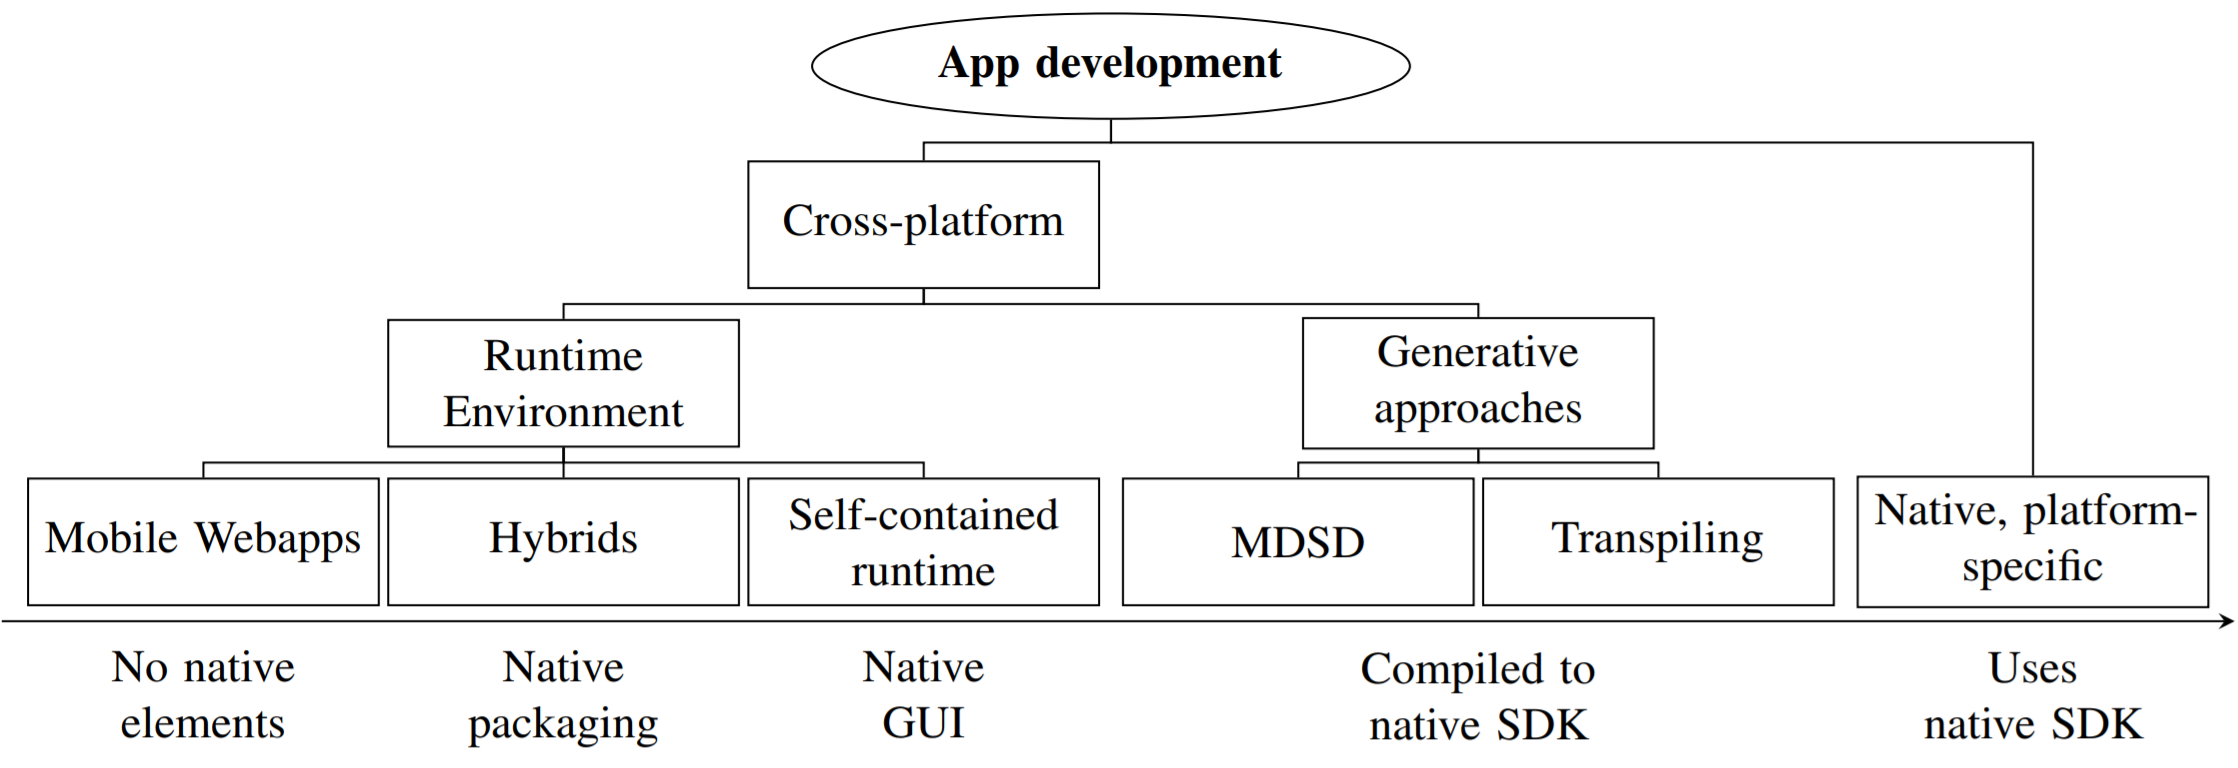
\includegraphics[scale=0.3]{kategorisierung_app_dev}
	\centering
	\caption[Kategorisierung von cross-plattform Entwicklungsansätzen]{Kategorisierung von cross-plattform Entwicklungsansätzen \cite{Majchrzak_category}}
	\label{fig:kategorisierung_app_dev}
\end{figure}

\newpage
\section{Native App-Entwicklung}

Die Native App-Entwicklung stellt zwar kein Framework dar, ist jedoch trotzdem wichtig zu erwähnen, da dies die ursprüngliche Art für ein mobiles Gerät zu entwickeln war und eine Referenz zu den folgenden Ansätzen darstellen soll.\\

Bei der nativen Entwicklung wird die Applikation mit den Technologien, Programmiersprachen und Tools entwickelt, welche von dem Hersteller der Zielplattform zur Verfügung gestellt wurden. Dafür wird ein \ac{SDK} genutzt, um die gewünschten Funktionen der Hardware zu benutzen und die passenden \ac{UI}-Elemente zu rendern und auf Eingaben des Nutzers zu reagieren. Jedoch ist der Quellcode an die jeweilige Zielplattform gebunden, da es sich um plattformspezifischen Bytecode handelt.
\begin{figure}[h]
	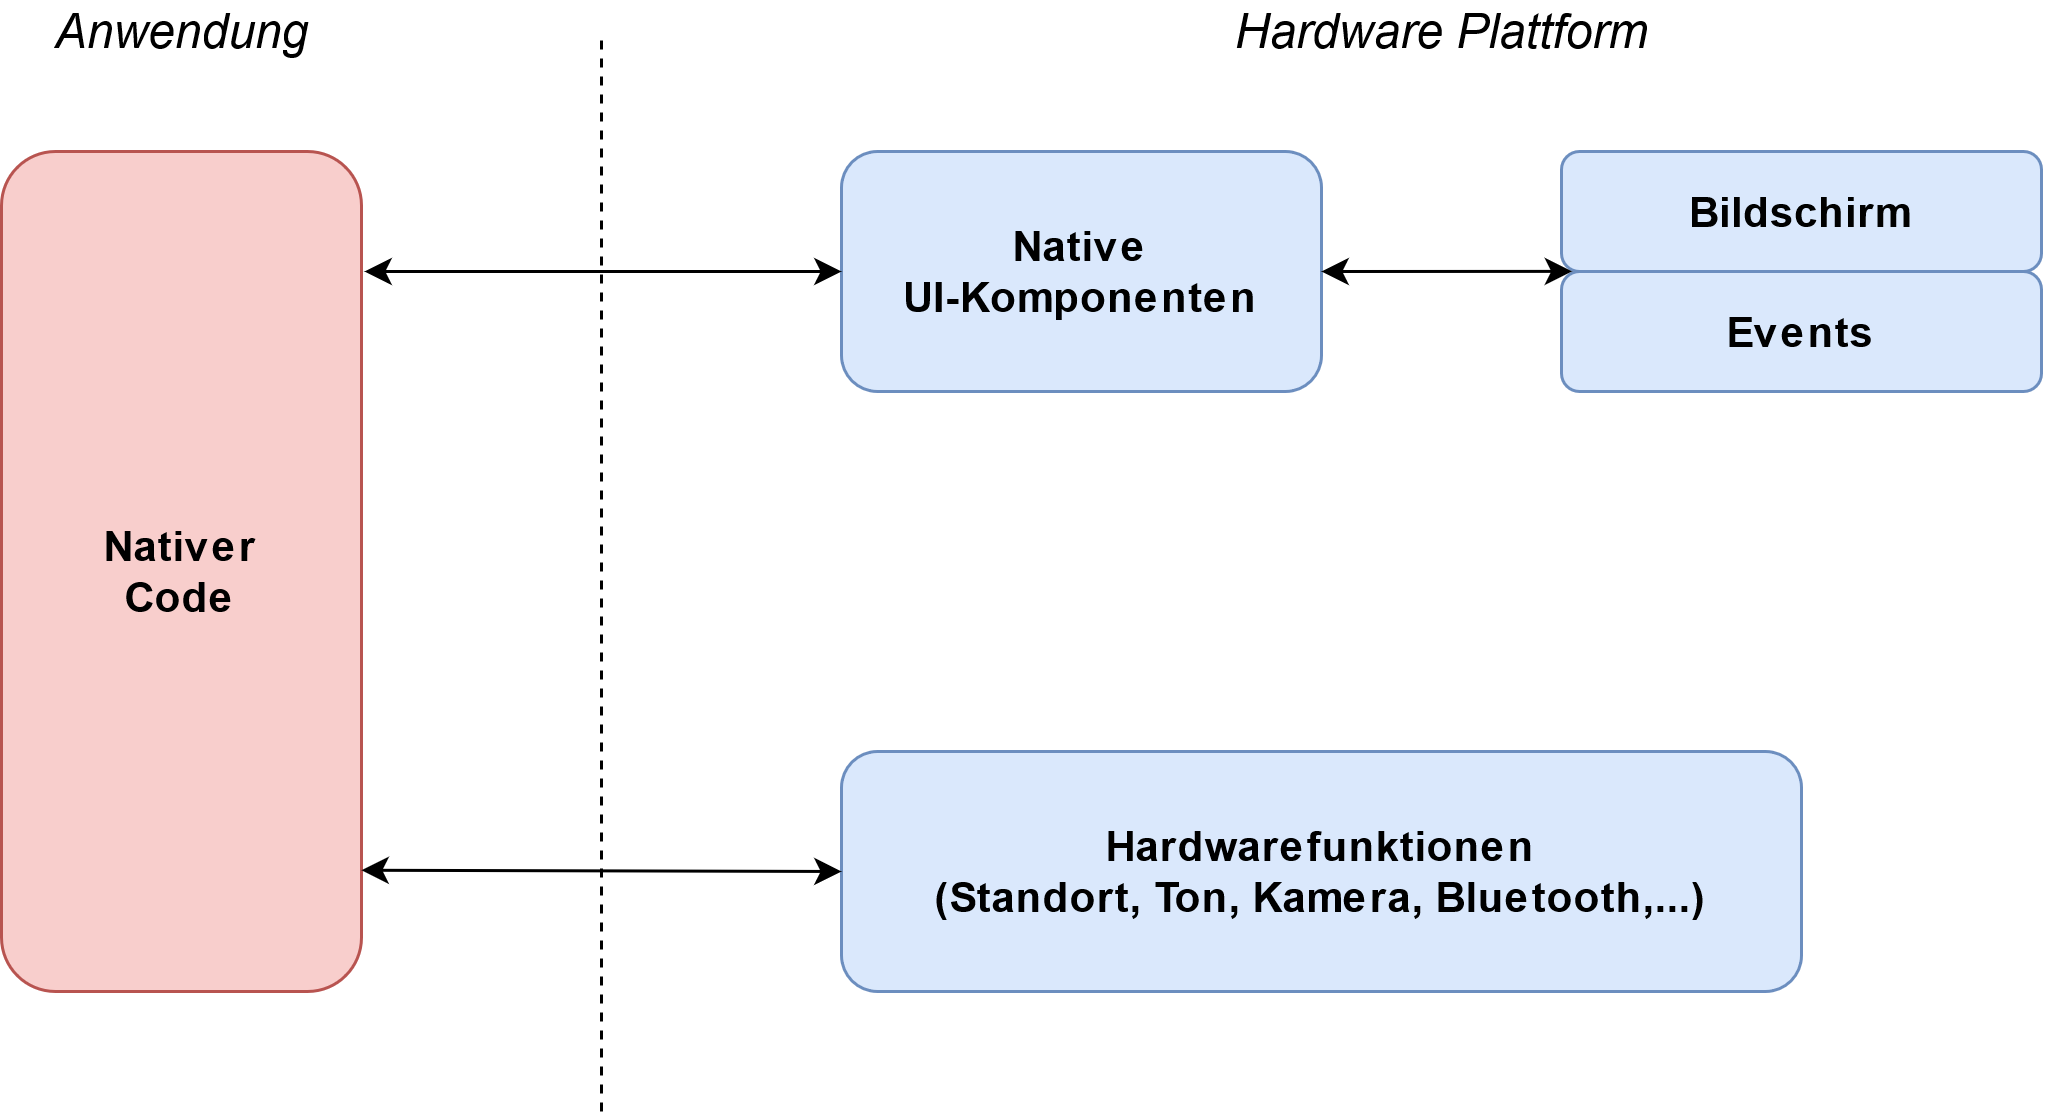
\includegraphics[scale=0.15]{native_framework}
	\centering
	\caption{Vereinfachtes Schema einer nativen Anwendung}
\end{figure}

Somit kann eine native Android Anwendung nur in Java oder Kotlin geschrieben werden, um zusammen mit dem Android \ac{SDK} die notwendige Funktionalität zu gewährleisten, während bei iOS Objective-C oder Swift benutzt werden muss, um zusammen mit Apples \ac{SDK} eine native Applikation zu erstellen\cite{rieger_evaluation}.\\

Die Native App wird anschließend im App-/Playstore des jeweiligen Betriebssystems veröffentlicht und kann von dort aus vom User heruntergeladen werden. Updates werden ebenfalls über diese Plattform verwaltet und dem User ausgespielt.

\makeatletter % Siehe https://tex.stackexchange.com/questions/19163/set-table-position-to-top
\setlength{\@fptop}{0pt}
\makeatother
\begin{table}[h]
	\begin{tabularx}{\linewidth}{>{\parskip1ex}X@{\kern4\tabcolsep}>{\parskip1ex}X}
		\toprule
		\hfil\bfseries Vorteile
		&
		\hfil\bfseries Nachteile
		\\\cmidrule(r{3\tabcolsep}){1-1}\cmidrule(l{-\tabcolsep}){2-2}
		
		%% PROS, seperated by empty line or \par
		Zugang zu allen Features der Zielplattform über die \ac{SDK} \ac{API}.\par
		Bestmögliche Performance auf dem Zielgerät, verglichen mit anderen Entwicklungsansätzen.\par
		Natives \glqq Look and Feel\grqq\  der \ac{UI}-Komponenten.\par
		Sofortiger Zugriff auf alle neuen Features der jeweiligen Zielplattform, sobald diese veröffentlicht werden.\par
		
		&
		
		%% CONS, seperated by empty line or \par
		Aufgrund der plattformspezifischen Tools muss dieselbe Applikation gleich zwei Mal entwickelt werden, was zu höherem Aufwand, längerer Entwicklungszeit, Notwendigkeit von zwei Entwicklungsteams mit Kenntnissen in verschiedenen Technologien und somit zu höheren Kosten führt.\par
		Native Apps sind komplexer in der Entwicklung und benötigen einen gewissen Grad an Erfahrung\cite{xanthopoulos_compare_cross_plattform}\par
		Einschränkungen und zusätzlichen Kosten, welche bei der Entwicklung und Veröffentlichung auf bestimmten Verteilungsplattformen entstehen. Da dies jedoch für jeden Ansatz gilt, welcher die App über den App-/Playstore verteilt wird dieser Aspekt im Folgenden nicht mehr explizit genannt.
		(Zugang zu Apples kostenpflichtigen Developer Program\cite{apple_member} und die Notwendigkeit eines Review-Prozesses von Apple, um eine App in dem App Store veröffentlichen zu können\cite{apple_submit})\par
		\\\bottomrule
	\end{tabularx}
	\caption{Vor- und Nachteile der nativen App-Entwicklung}
\end{table}

\clearpage
\section{Auf einer Laufzeitumgebung basierende Ansätze}
Bei dieser Oberkategorie an mobile App Frameworks wird eine Laufzeitumgebung genutzt, um eine übergeordnete Abstraktion der darunterliegenden Plattform zu schaffen. Somit können Anwendungen, welche darauf aufbauen eine einheitliche Schnittstelle verwenden und können somit Plattformübergreifend genutzt werden.
Diese Ansätze werden anhand der dafür genutzten Laufzeitumgebung weiter unterteilt.


\subsection{(Progressive) Web-App}

\subsubsection{\glqq Klassische\grqq\  Web-App}

Eine Web-App stellt eine Art einer Anwendung dar, welche innerhalb eines Browsers auf einem mobilen Gerät ausgeführt wird und mithilfe von Web-Technologie wie \ac{HTML}, \ac{CSS} und JavaScript erstellt wurde. Diese sind über einer \ac{URL} erreichbar und basieren, wie jede Website, auf dem klassischen Client-Server-Modell. Somit ist die Web-App komplett betriebssystemunabhängig, da lediglich ein aktueller Browser und eine Internetverbindung notwendig sind, um diese auf einem Endgerät zu nutzen. Dieser stellt somit die Laufzeitumgebung bereit, in der die Applikation ausgeführt wird. Dieser kümmert sich um die Darstellung und Verarbeitung von Inputs des Benutzers. Dabei werden keine nativen Features, welche über die Möglichkeiten des Browsers verwendet und es werden ebenfalls keine nativen \ac{UI}-Komponenten benutzt.\cite{waffa_tax_dev_approaches}.

\begin{figure}[h]
	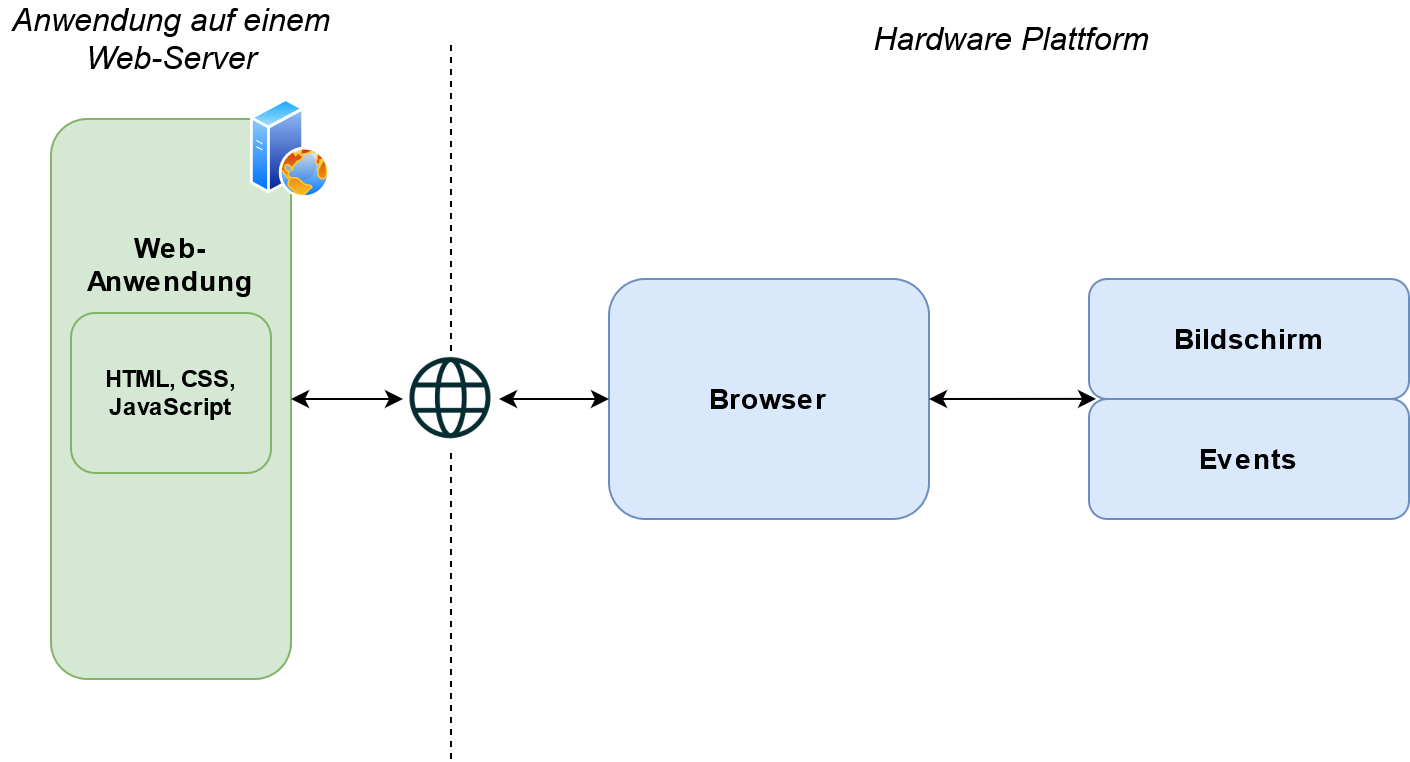
\includegraphics[scale=0.23]{web_app}
	\centering
	\caption{Vereinfachtes Schema einer Web-Anwendung}
\end{figure}

\begin{table}[h]
	\begin{tabularx}{\linewidth}{>{\parskip1ex}X@{\kern4\tabcolsep}>{\parskip1ex}X}
		\toprule
		\hfil\bfseries Vorteile
		&
		\hfil\bfseries Nachteile
		\\\cmidrule(r{3\tabcolsep}){1-1}\cmidrule(l{-\tabcolsep}){2-2}
		
		%% PROS, seperated by empty line or \par
		Die Verarbeitung geschieht auf einem Web-Server, sodass nur die \ac{UI}-Elemente an das Endgerät geschickt werden.\par
		Die Wartung der Anwendung ist leichter, da diese nur auf dem Web-Server liegt.\par
		Dieselbe Anwendung kann direkt in Browsern verschiedener Endgeräte angezeigt werden.\par
		
		&
		
		%% CONS, seperated by empty line or \par
		Sind nicht im App-/Playstore verfügbar.\par
		Eine Internetverbindung ist zwingend erforderlich.\par
		Schwächere Performance, da in einem Browser ausgeführt.\par
		Browserkompatibilität nicht überall gewährleistet.\par
		Keinen Zugriff auf alle Hardwarefunktionen, sondern sind auf die des Browsers beschränkt.\par
		\\\bottomrule
	\end{tabularx}
	\caption{Vor- und Nachteile einer \glqq klassischen\grqq\ Web-App}
\end{table}

\newpage
\subsubsection{Progressive Web-App}

Der Name Progressive Web-App ist kein allgemein definierter Begriff. Dieser wurde 2015  von dem Google Entwickler Alex Russell eingeführt, um eine sich an das Endgerät anpassende Web-Applikation zu beschreiben, welche ausschließlich aus Web-Technologien wie unter anderem JavaScript, \ac{CSS} und \ac{HTML} besteht. Zusätzlich erweitert die \ac{PWA} den Funktionsumfang einer Web-App um Verhaltensweisen und Features, welche Traditionell den nativen Apps vorbehalten waren. Dazu gehören u.A. das Hinzufügen zu dem Homescreen, eine Möglichkeit die Website auch ohne Internet zu bedienen, und Push-Benachrichtigungen zu erhalten\cite{mozilla_pwa}. Besonders hervorzuheben ist die Tatsache, dass der User selbst entscheidet, ob diese Features genutzt werden sollen oder nicht. 

\blockcquote{firtman_mobile_web}{
	A PWA is a Website running in a browser that will progressively add more features based on compatibility.
}


Dabei stellt die Progressive Web-App keine einzige Technologie dar, sondern eher eine Ansammlung an Eigenschaften, welche erfüllt werden sollten, um als eine \ac{PWA} bezeichnet werden zu können. Die Kriterien welche Google für eine \ac{PWA} nennt sind in zwei Kategorien aufgeteilt. Kernanforderungen an die Website und Zusatzanforderungen welche eine \glqq optimale\grqq\ \ac{PWA} ausmachen.\\


\begin{table}[!h]
	\begin{tabularx}{\linewidth}{>{\parskip1ex}X@{\kern4\tabcolsep}>{\parskip1ex}X}
		\toprule
		\hfil\bfseries Kernanforderungen
		&
		\hfil\bfseries Zusätzliche Anforderungen
		\\\cmidrule(r{3\tabcolsep}){1-1}\cmidrule(l{-\tabcolsep}){2-2}
		
		%% Kernanforderungen, seperated by empty line or \par
		Geschwindigkeit\par
		Erreichbarkeit von jedem Browser und Endgerät\par
		Responsive Anpassung an die Bildschirmgröße\par
		Offline-Funktionalität\par
		Installierbarkeit\par
		
		&
		
		%% zusätzliche Anforderungen, seperated by empty line or \par
		Barrierefreiheit\par
		Sicherheit\par
		Sichtbarkeit (z.B. über Googles Suchfunktion)\par
		Transparenz bezüglich der erforderlichen Berechtigungen\par
		\\\bottomrule
	\end{tabularx}
	\caption[Anforderungen an eine \ac{PWA}]{Anforderungen an eine \ac{PWA}\cite{google_pwa_check}}
\end{table}

\newpage
Zu den technischen Bestandteilen, welche eine \ac{PWA} von einer Web-App unterscheiden gehören:\\

\begin{enumerate}
	\item Die App Shell - Stellt das minimale \ac{HTML}, \ac{CSS} und JavaScript Gerüst dar, in welchem der Content der \ac{PWA} angezeigt werden soll. Sie ist dafür zuständig die statischen Inhalte der Anwendung anzuzeigen, welche im Nutzungsverlauf der \ac{PWA} gleich bleiben. Dazu gehört üblicherweise die Navigationsleiste oder die Homepage. Diese werden lokal auf dem Endgerät abgelegt, sodass Ladezeiten minimiert werden können.
	
	\item Der Service Worker - Ein Hintergrunddienst in JavaScript geschrieben, welcher auch bei geschlossener App weiterläuft. Dieser wird beim Abruf der \ac{PWA} mitgeliefert und genutzt, falls die \ac{PWA} \glqq zum Homescreen hinzugefügt\grqq\ wird. Er hat die Aufgabe Netzwerkanfragen abzufangen und passend zu verarbeiten. Außerdem verwaltet der Service Worker den Cache, wodurch Anfragen auch ohne Internet verarbeitet und beantwortet werden können, um die offline Funktionalität zu ermöglichen. Laut Biørn-Hansen et. al., 2017\cite{hansen_pwa} kann eine \ac{PWA} ohne Service Worker nicht richtig funktionieren. Damit ist der Service Worker der zentrale Bestandteil einer \ac{PWA}. 
	
	\item Das Web Application Manifest - 
	Eine Datei, welche es dem Entwickler ermöglicht das Verhalten und Aussehen der \glqq installierten\grqq\ \ac{PWA} auf dem mobilen Gerät des Users anzupassen. Dazu gehören u.A. das angezeigte Logo auf dem HomeScreen oder verschiedenen Caching-Strategien.
	
\end{enumerate}

\begin{figure}[!ht]
	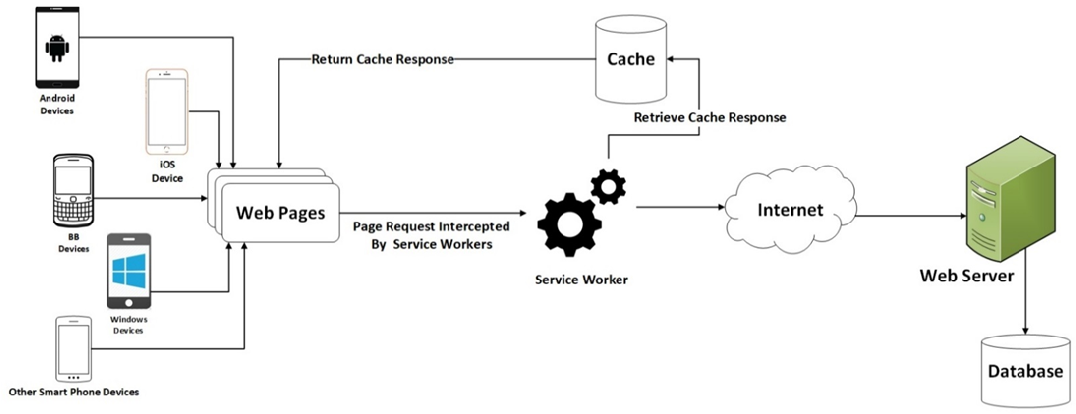
\includegraphics[scale=0.45]{pwa_aufbau}
	\centering
	\caption[Technischer Aufbau einer \ac{PWA}]{Technischer Aufbau einer \ac{PWA} \cite{adetunji_pwa}}
\end{figure}


\begin{table}[ht!]
	\begin{tabularx}{\linewidth}{>{\parskip1ex}X@{\kern4\tabcolsep}>{\parskip1ex}X}
		\toprule
		\hfil\bfseries Vorteile
		&
		\hfil\bfseries Nachteile
		\\\cmidrule(r{3\tabcolsep}){1-1}\cmidrule(l{-\tabcolsep}){2-2}
		
		%% PROS, seperated by empty line or \par
		Eine \ac{PWA} lässt sich auch ohne Internetverbindung benutzen.\par
		Die \ac{PWA} ist leicht erreichbar und teilbar, da diese über einen Link im Browser abgerufen werden kann.\par
		Es ist möglich bereits bestehende Webseite zu einer \ac{PWA} umzuwandeln.\par
		Funktionen wie \glqq zum Homescreen hinzugefügen\grqq\ oder Push-Benachrichtigungen führen dazu, dass der Nutzer die Web-App als native Anwendung wahrnimmt und anders mit dieser interagiert\cite{medium_pwa_pro_con}.\par
		Eine \ac{PWA} benötigt zwingend \ac{HTTPS}, was die Datenübertragung vor \glqq man-in-the-middle\grqq\ Attacken zusätzlich schützt.\par
		
		&
		
		%% CONS, seperated by empty line or \par
		\ac{PWA}s haben keinen Zugriff auf alle Hardwarefunktionen, sondern sind auf die des Browsers beschränkt.\par
		Sind nicht im App-/Playstore verfügbar.\par
		Schwächere Performance, da in einem Browser ausgeführt.\par
		\ac{PWA}s sind derzeit noch nicht auf allen Geräten und Browsern komplett unterstützt.\par
		\\\bottomrule
	\end{tabularx}
	\caption[Vor- und Nachteile einer \ac{PWA}]{Vor- und Nachteile einer \ac{PWA}\cite{adetunji_pwa}}
\end{table}

\clearpage
\subsection{Hybride App}

Hybride Apps stellen eine Kombination von Web-Apps und nativen Apps dar. Diese verwenden, ebenfalls vorwiegend Web-Technologien. Der Quelltext  wird ebenfalls innerhalb eines Browsers ausgeführt. Jedoch handelt es sich dabei nicht um den bereits installierten Browser wie bei Web-Apps, sondern um einen plattformspezifischen Container (UIWebView unter iOS und WebView unter Android)\cite{xanthopoulos_compare_cross_plattform}. Dieser wird bei dem Download der App aus dem App-/Playstore zusammen mit dem Quellcode der App im Hintergrund bereitgestellt und stellt die Laufzeitumgebung dar. Die \ac{UI}-Komponenten werden weiterhin von dem Container gerendert, obwohl manche Frameworks versuchen diese möglichst nativ aussehen zu lassen. Um die Limitierungen des Zugriffes auf bestimmte Hardware oder Informationen aus dem Browser heraus zu umgehen, wird mithilfe eines \grqq Überbrückungs-Moduls\grqq\ auf den nativen Teil der Anwendung zugegriffen. Dieser hat Zugriff auf die nativen APIs der Plattform. Dies führt, je nachdem wie aktive diese verwendet wird, zu einem Performance-Engpass, welcher in \foreignlanguage{ngerman}{\cref{react}} näher erläutert wird. Jedoch ist dieser Teil der Hybriden App wiederum plattformspezifisch. Allerdings stellen cross-plattform Frameworks diese Funktionalität direkt bereit und nehmen dem Entwickler viel Arbeit ab, sodass es bei der Entwicklung selten notwendig ist nativen Code selbst zu schreiben\cite{kmu_fh_joanneum}.

\begin{figure}[!h]
	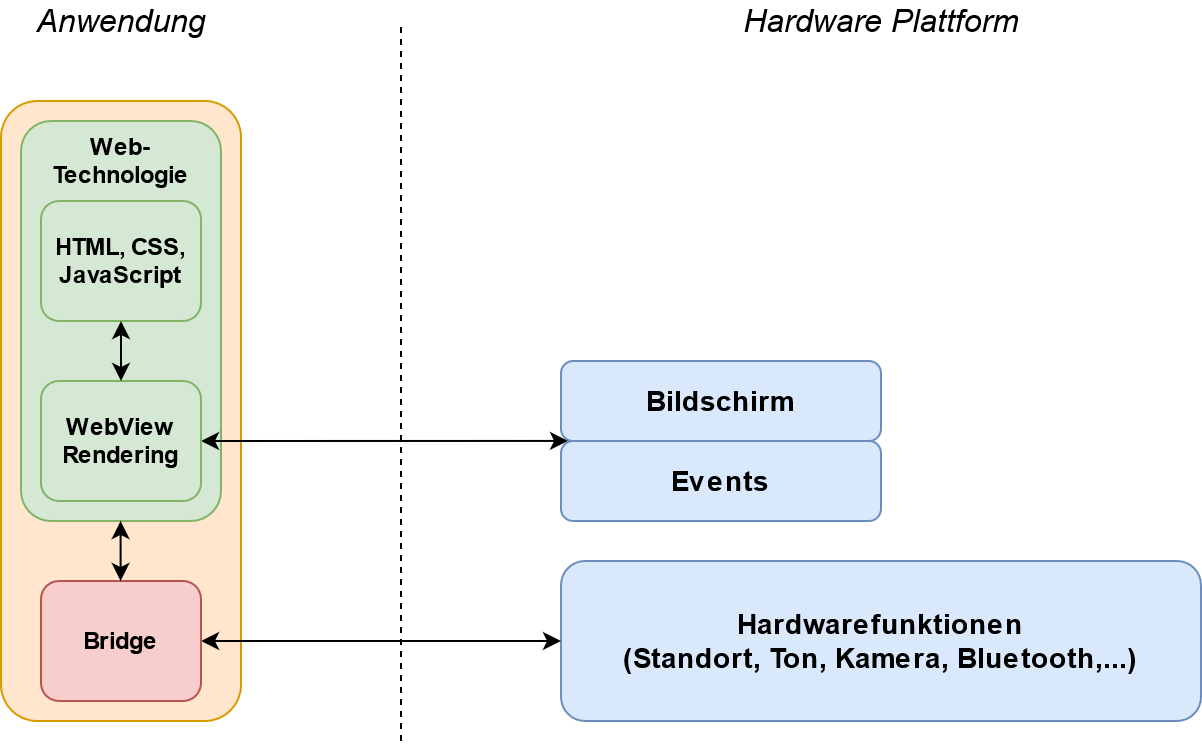
\includegraphics[scale=0.25]{hybrid_app}
	\centering
	\caption{Vereinfachtes Schema einer hybriden App}
\end{figure}

\begin{table}[!h]
	\begin{tabularx}{\linewidth}{>{\parskip1ex}X@{\kern4\tabcolsep}>{\parskip1ex}X}
		\toprule
		\hfil\bfseries Vorteile
		&
		\hfil\bfseries Nachteile
		\\\cmidrule(r{3\tabcolsep}){1-1}\cmidrule(l{-\tabcolsep}){2-2}
		
		%% PROS, seperated by empty line or \par
		Kann über den App-Store verteilt werden, sowie als Web-App bereitgestellt werden.\par
		Für die Implementierung und Tests kann größtenteils der Desktop-Browser genutzt werden.\par
		Hat Zugriff auf vom Framework unterstützten Hardwarefunktionen.\par
		Die Anwendung hat auf verschiedenen Endgeräten ein einheitliches \ac{UI}/\ac{UX}, da der Inhalt mit Web-Technologie definiert und in einem browserähnlichem Container dargestellt wird.\par
		Eine bereits bestehende Webseite kann in kurzer Zeit zu einer hybriden App umgewandelt werden.\par
		
		&
		
		%% CONS, seperated by empty line or \par
		Schwächere Performance, da die App innerhalb einer Browser-Engine ausgeführt wird und manipulationen des \ac{DOM}s viel Zeit kosten.\par
		Häufige Nutzung nativer Funktionen kann ebenfalls die Performance beeinflussen.\par
		Mehr Fehlerquellen durch Nutzung verschiedener Technologien, welche sich je nach Plattform unterschiedlich verhalten kann.\par
		Kein Zugriff auf native \ac{UI}-Elemente.\par
		\\\bottomrule
	\end{tabularx}
	\caption{Vor- und Nachteile einer hybriden App}
\end{table}

\clearpage %Macht komische freistellen siehe https://tex.stackexchange.com/questions/2958/why-is-newpage-ignored-sometimes
\subsection{Eigenständige Laufzeitumgebung}

Im Gegensatz zu der (progressiven) Web-App und dem hybriden Ansatz greift diese Art der Anwendung nicht mehr auf die üblichen Web-Technologien zurück und rendert den Inhalt nicht innerhalb eines Browsers oder browserähnlichen Containers, sondern stellt eine vollständig eigenständige Laufzeitumgebung zur Verfügung. Somit wird es den Entwicklern der Applikation ermöglicht Programmiersprachen wie JavaScript (z.B. React Native) oder C\# (z.B. Xamarin) zu verwenden. Um das Übersetzen der Aufrufe aus dem plattformunabhängigen Quellcode in das passende native Äquivalent kümmert sich ein \grqq Überbrückungs-Modul\grqq\ oder \ac{API} des Frameworks. Dies führt jedoch, je nach Verwendungshäufigkeit, ebenfalls zu einem Performance-Engpass, welcher in \foreignlanguage{ngerman}{\cref{react}} näher erläutert wird. Die Laufzeitumgebung deckt somit einen größeren Aufgabenbereich als der hybride Ansatz ab und ist somit flexibler, da hierbei das Rendern der \ac{UI} mit nativen Elementen realisiert werden kann.\cite{hansen_performance_overhead_cross_platform}


\begin{figure}[!h]
	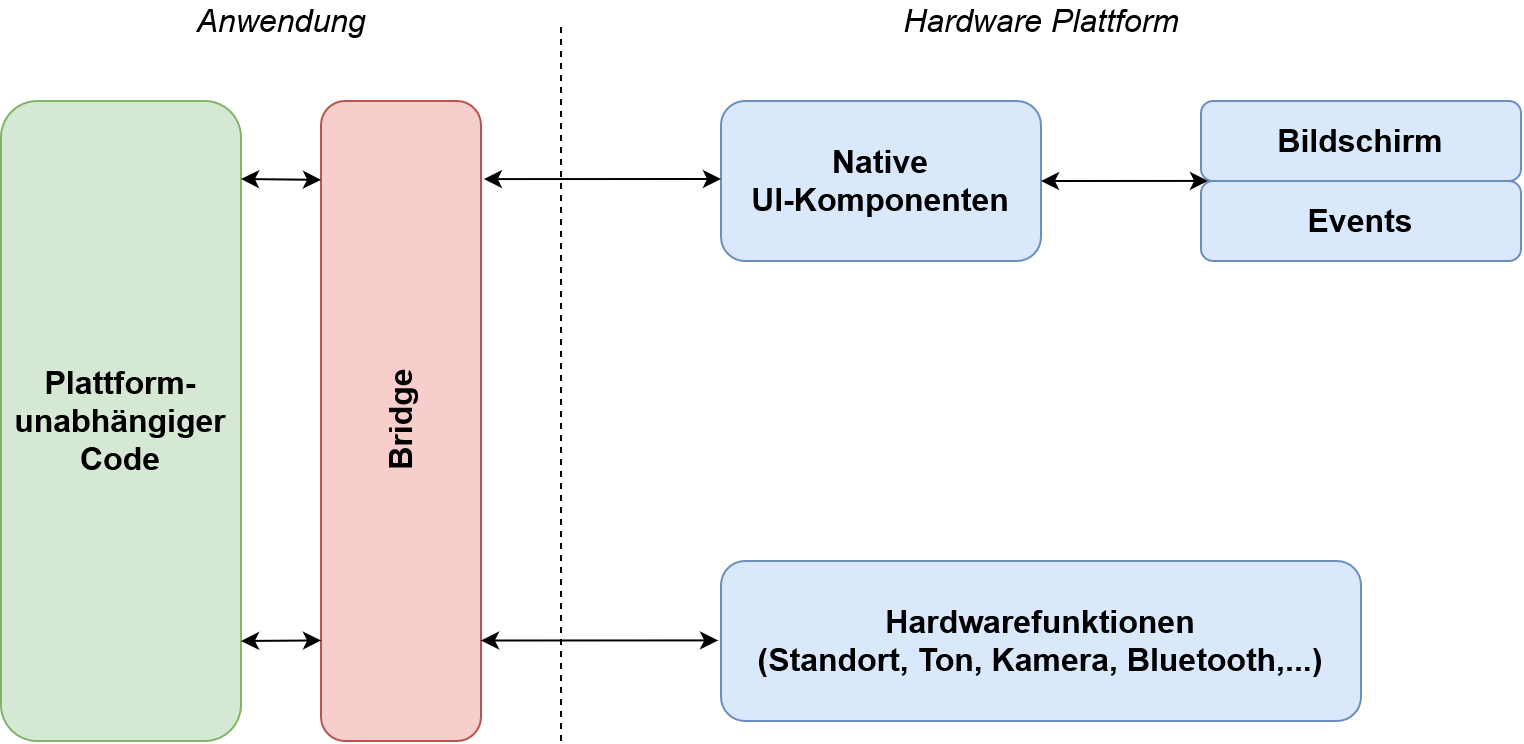
\includegraphics[scale=0.21]{eigenstaendige_laufzeitumgebung}
	\centering
	\caption{Vereinfachtes Schema einer App mit eigener Laufzeitumgebung}
\end{figure}


\begin{table}[h]
	\begin{tabularx}{\linewidth}{>{\parskip1ex}X@{\kern4\tabcolsep}>{\parskip1ex}X}
		\toprule
		\hfil\bfseries Vorteile
		&
		\hfil\bfseries Nachteile
		\\\cmidrule(r{3\tabcolsep}){1-1}\cmidrule(l{-\tabcolsep}){2-2}
		
		%% PROS, seperated by empty line or \par
		Es besteht kein Zwang Web-Technologien verwenden zu müssen.\par
		Die Anwendung kann über den App-/Playstore verteilt werden.\par
		Es können native \ac{UI}-Elemente verwendet werden.\par
		Es sind vom Framework unterstützten Hardwarefunktionen verfügbar.\par
		
		&
		
		%% CONS, seperated by empty line or \par
		Komplexe Frameworks, da diese mehrere verschiedene Aufgaben übernehmen.\par
		Je nach Kenntnisstand höherer Einarbeitungsaufwand.\par
		Performance leidet unter der Notwendigkeit mit nativen Komponenten über die Bridge kommunizieren zu müssen.\par
		Initiale Startzeit der App ist hoch, da aufgrund der erhöhten Komplexität eine größere Codebasis interpretiert und \ac{JIT} kompiliert werden muss.\par
		\\\bottomrule
	\end{tabularx}
	\caption{Vor- und Nachteile einer App mit eigenständiger Laufzeitumgebung}
\end{table}

\newpage
\section{Generierende Ansätze}

Bei diesen Ansätzen wird es dem Entwickler ermöglicht eine Applikation einmalig zu entwickeln und daraus nativen Code für die jeweilige Zielplattform zu generieren.
Dabei wird zwischen modellgetriebenen und cross-kompilierenden Ansätzen weiter unterschieden.

\subsection{Modellgetrieben}

Bei diesem Ansatz wird die Applikation in einer Modellierungssprache (Textuell oder Grafisch) plattformunabhängig definiert.
Hierbei kann wiederum in zwei Gruppen unterteilt werden: Mehrstufig und einstufig generierende Ansätze. \\

Bei der Einstufigen Code Generation wird aus der Modellierungssprache mit Hilfe von mehreren Codegeneratoren nativer Quellcode für die jeweilige Zielplattform erzeugt. Beispiele dafür wären MD2, MobML oder Mobl.\\

Bei der Mehrstufigen Code Generation wird Quellcode für ein weiteres Cross-Plattform Framework erzeugt. Daraus wird in einem weiteren Schritt wiederum Quellcode für die jeweilige Zielplattform erzeugt. Ein Beispiel für solch ein Framework wäre AXIOM.\\

Diese Ansätze sind jedoch als Spezialfälle zu betrachten und werden vorwiegend akademisch Diskutiert. Kommerzielle Ansätze existieren haben jedoch alle eigene Modellierungssprachen, wodurch sich diese Ansätze nicht durchsetzen konnten\cite{umuhoza_modell}\cite{hansen_performance_overhead_cross_platform}.\\

\begin{table}[h]
	\begin{tabularx}{\linewidth}{>{\parskip1ex}X@{\kern4\tabcolsep}>{\parskip1ex}X}
		\toprule
		\hfil\bfseries Vorteile
		&
		\hfil\bfseries Nachteile
		\\\cmidrule(r{3\tabcolsep}){1-1}\cmidrule(l{-\tabcolsep}){2-2}
		
		%% PROS, seperated by empty line or \par
		Definition der Applikation auf einem sehr hohen und abstrakten Level möglich.\par
		Keine Notwendigkeit Code zu schreiben.\par
		Sehr hohe Entwicklungsgeschwindigkeit bei Entwicklung von Prototypen möglich.\par

		&
		
		%% CONS, seperated by empty line or \par
		Zersplitterte Framework-Landschaft.\par
		Fehleranfällig, da viele verschiedene Technologien aufeinander aufbauen.\par
		Können häufig nur die Features anbieten, welche auf allen Plattformen verfügbar sind.\par
		Kleine Community und wenig Hilfsmaterialien, daher vorwiegend akademisch Diskutiert.\par
		
		\\\bottomrule
	\end{tabularx}
	\caption{Vor- und Nachteile einer modellgetriebenen App}
\end{table}


\newpage
\subsection{Cross-Kompilierend}

Bei diesem Ansatz wird versucht den geschrieben Quellcode der Anwendung in eine, für die Zielplattform passende Repräsentation umzuwandeln. Dies kann auf verschiedenen Abstraktionsebenen des Quellcodes geschehen. Daher wird in der Literatur der Begriff kompilierend oder transpilierend benutzt. Bei der Kompilation wird meist Quellcode einer niedrigeren Abstraktionsstufe erzeugt wird, während bei der Transpilation Quellcode häufig auf ähnlicher Abstraktionsstufe erzeugt wird. Diese Trennung ist jedoch nicht einheitlich definiert und ist daher häufig kontextabhängig. Allerdings fokussieren sich solche Ansätze die Regel nur auf einen bestimmten Aspekt der Anwendung, sodass noch zusätzliche Schritte notwendig sind, um eine vollständige App zu erzeugen. Ein Beispiel dafür ist Googles J2ObjC \cite{hansen_performance_overhead_cross_platform}.
Besonders hervorzuheben ist dabei Googles Flutter Framework, bei welchem die Applikation in Dart geschrieben wird. Dieses ist der jüngste Vertreter dieser Kategorie. Eine Besonderheit bei Flutter besteht darin, dass keine Nativen Komponenten gerendert werden. Das Framework überlässt diese Aufgabe komplett der mitgelieferten Skia Graphics Engine. Daraus folgt eine erhöhte Flexibilität und Performance\cite{medium_rendering_flutter}. \\

\begin{table}[h]
	\begin{tabularx}{\linewidth}{>{\parskip1ex}X@{\kern4\tabcolsep}>{\parskip1ex}X}
		\toprule
		\hfil\bfseries Vorteile
		&
		\hfil\bfseries Nachteile
		\\\cmidrule(r{3\tabcolsep}){1-1}\cmidrule(l{-\tabcolsep}){2-2}
		
		%% PROS, seperated by empty line or \par
		Ähnliche Performance zu nativen Apps möglich.\par
		Es können native \ac{UI}-Elemente verwendet werden.\par
		
		&
		
		%% CONS, seperated by empty line or \par
		Es werden, je nach Framework, nur eine Begrenze Anzahl an Plattformen unterstützt.\par
		Es werden nur Features unterstützt, welche auf allen Plattformen verfügbar sind.\par
		Legen den Fokus teilweise nur auf einen bestimmten Aspekt der Anwendung, sodass noch weitere Schritte notwendig sind, um eine vollwertige App zu erzeugen.\par
		\\\bottomrule
	\end{tabularx}
	\caption{Vor- und Nachteile einer cross-kompilierenden App}
\end{table}
	\chapter{Framework Beispiele}

\section{Auswahlkriterien}

Im Folgenden wird auf einige ausgewählte Frameworks konkret eingegangen, welche auf verschiedenen Ansätzen beruhen. Dabei wurde der native Ansatz nicht mit in die nähere Betrachtung aufgenommen, da dieser nicht plattformunabhängig ist. Ebenso wurden \ac{PWA}s nicht weiter berücksichtigt, da deren Möglichkeiten Browserabhängig sind. Zunächst wurde eine Literaturrecherche durchgeführt bei der folgende Frameworks häufig genannt wurden:

\begin{multicols}{3}
	\begin{itemize}
		\vspace{-2mm}
		\setlength\itemsep{0mm}
		\item Titanium
		\item Sencha Touch
		\item Corona SDK
		\item PhoneGap
		\item Native Script
		\item Xamarin
		\item Ionic
		\item React Native
		\item Flutter
	\end{itemize}
\end{multicols}



Um die Relevanz und Aktivität der Community jener Frameworks zu bewerten, wurde das StackOverflow-Trends Tool \footnote{https://insights.stackoverflow.com/trends} genutzt. Dieses zeigt die relative Verteilung der gestellten Fragen zu bestimmten Technologien im Zeitverlauf.

\begin{figure}[h]
	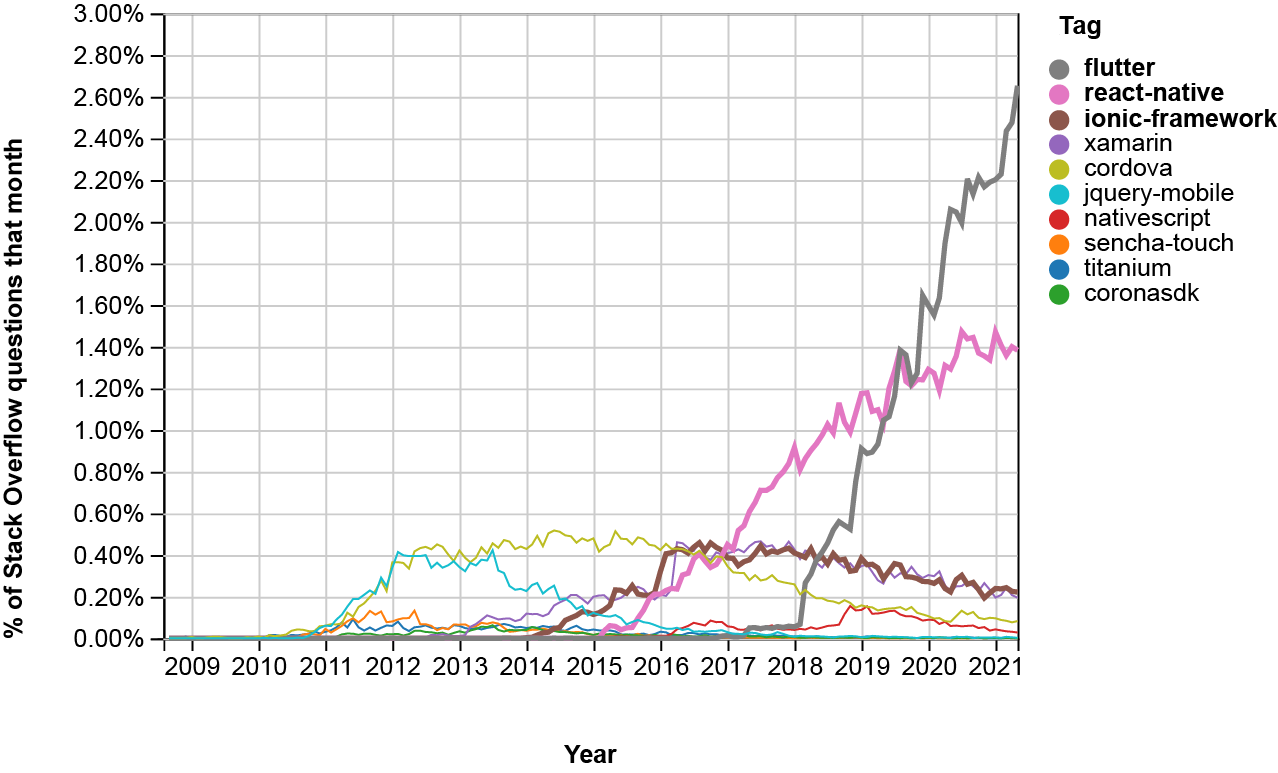
\includegraphics[scale=0.5]{framework_trends}
	\centering
	\caption{Verteilung der gestellten Fragen auf StackOverflow ausgewählter Frameworks}
\end{figure}

Auf dieser Grundlage wurden die drei populärsten Frameworks ausgewählt auf die im Folgenden näher eingegangen wird.

\newpage

\section{Das Hybride Framework Ionic}

Ionic ist ein Open Source cross-plattform Framework welches 2013 von dem Startup Drifty veröffentlicht wurde. Eine Ionic App nutzt Web-Technologien wie \ac{HTML}, \ac{CSS}, TypeScript und baut auf AngularJS und Apache Cordova auf\cite{wiki_intro}. \\

Es kann flexibel für hybride Apps und \ac{PWA}s verwendet werden. Der Fokus von Ionic liegt auf dem Frontend. Zunächst aufbauend auf dem Angular Framework stellt Ionic \ac{UI}- Komponenten für z.B. Listen, Buttons, Layouts bereit, welche den nativen Gegenstücken nachempfunden sind. Technisch bildet dabei Apache Cordova die Schnittstelle für plattformspezifische Funktionalitäten als auch die Grundlage, um plattformunabhängige Applikationen erstellen zu können. Seit Version 4 ist Ionic nicht mehr fest an AngularJS gekoppelt und es können beliebige Front-End-Frameworks wie React oder Vue benutzt werden, sowie Ionics eigene Komponenten, ohne spezifisches Front-End-Framework. Außerdem kann statt Apache Cordova Ionics eigene Laufzeitumgebung Capacitor genutzt werden, um die Anwendung auf einem Endgerät auszuführen\cite{ionic_docs}\cite{ionic_intro}.\\

	\begin{figure}[h]
		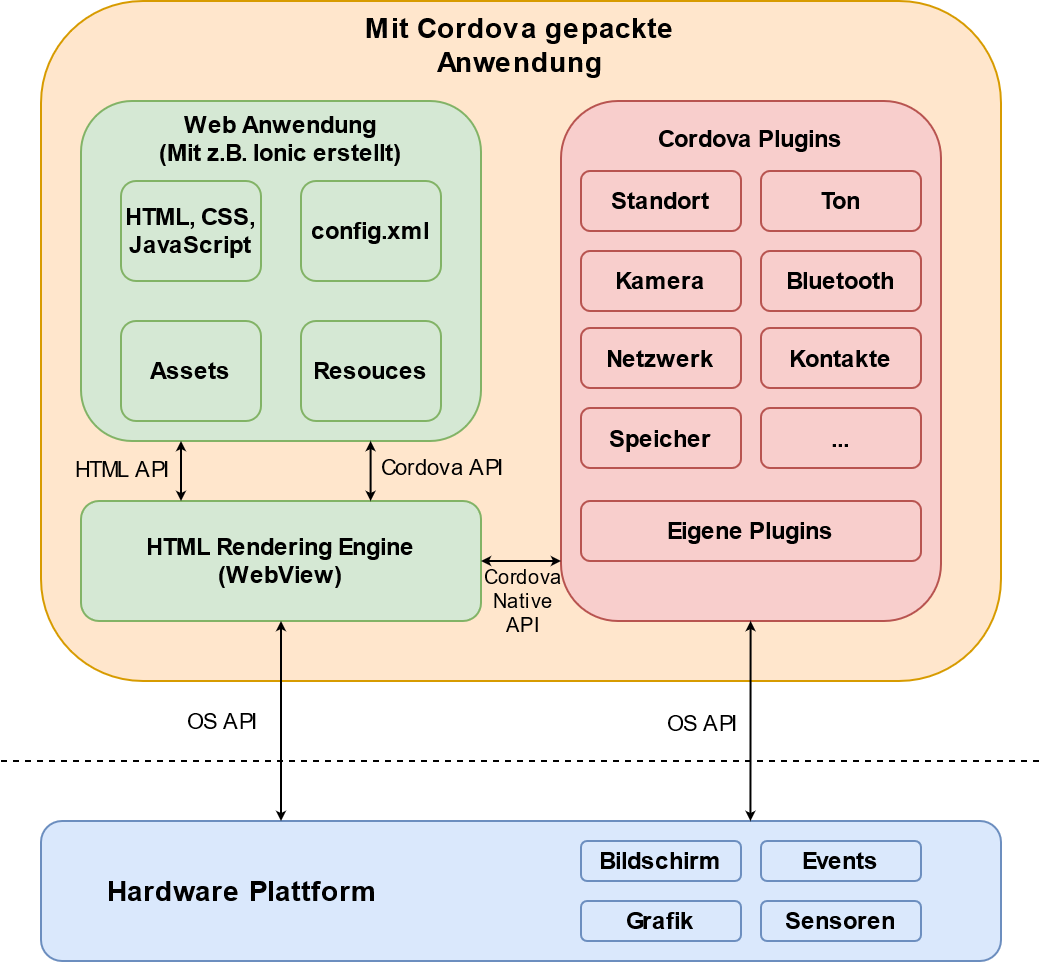
\includegraphics[scale=0.25]{cordova_ionic}
		\centering
		\caption[Übersicht einer mit Cordova gepackten App]{Übersicht einer mit Cordova gepackten App (Anlehnung an \cite{cordova_diagramm} )}
	\end{figure}

\newpage

Die Komponenten der Applikation werden mit \ac{HTML} definiert, mit \ac{SASS}, einem Superset von \ac{CSS} mit Zusatzfunktionen, gestyled und deren verhalten mit JavaScript oder optional mit TypeScript definiert. Die Sprache TypeScript wurde von dem Angular Framework übernommen und stellt ein Superset von JavaScript dar, welche einige zusätzliche Sprachfeatures als auch ein Typsystem bietet. Die mit TypeScript definierten Komponenten werden zu JavaScript tanspiliert, sodass Typfehler während des Kompilierens identifiziert werden können. Die mit Ionic gebauten Anwendungen können über die Plattform spezifischen App-Stores ausgeliefert, oder als Web-App verfügbar gemacht werden.

\begin{figure}[h]
	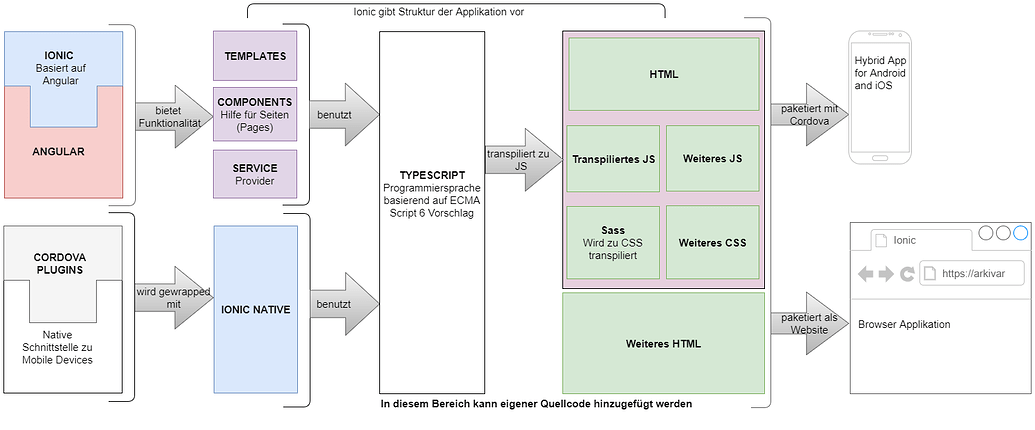
\includegraphics[scale=0.46]{ionic_flow_arkivar}
	\centering
	\caption[Übersicht der verwendeten Technologien einer Ionic App]{Übersicht der verwendeten Technologien einer Ionic App\cite{ionicForum_diagramm}}
\end{figure}

Werden bei der Entwicklung die angebotenen Komponenten genutzt, entsteht ein einheitliches Design, zudem ein umfassendes Theming viele Aspekte der Gestaltung bereits abnimmt. Jedoch kann dies auch zu einem Nachteil werden, vor allem dann, wenn Abweichungen von den Standardkomponenten gefordert sind. Ebenfalls als Nachteil ist hierbei die Performance von Ionic zu nennen, da im Gegensatz zu anderen Frameworks welche native \ac{UI}-Komponenten verwenden, diese hierbei im WebView gerendert werden\cite{altexsoft_comparison}.

\newpage
\section{React Native - Framework mit eigenständiger Laufzeitumgebung}
\label{react}
React Native wurde 2013 während eines Facebook internen Hackathon entwickelt und im Mai 2015 veröffentlicht, wobei zunächst nur iOS unterstützt wurde. Die Android-Unterstützung folgte wenige Monate später. React Native baut auf der \ac{API} des populären und ebenfalls von Facebook entwickelten JavaScript Framework React auf. Dieses wurde 2013 für Web-Anwendungen entwickelt und legt den Fokus auf die Darstellung von Komponenten abhängig von den zur Verfügung gestellten Daten des Anwenders oder der Anwendung. React Native übernimmt die Prinzipien von ReactJS, sodass jemand der mit ReactJS vertraut ist ohne Probleme auf React Native umsteigen könnte. Die gesamte Anwendung, zusammen mit den \ac{UI}-Komponenten wird mit JavaScript oder optional TypeScript, zusammen mit der eigenen Templating Syntax JSX geschrieben. React Native stellt in erster Linie abstrakte \ac{UI}-Komponenten bereit, welche anschließend auf das jeweilige Gegenstück der Zielplattform abgebildet werden. Somit kann eine Button-Komponente, wie jede andere React-Komponente, direkt in dem JavaScript Code importiert und verwendet werden. Diese hat auf der entsprechenden Plattform ein natives Gegenstück, welches gerendert wird\cite{rieger_evaluation}\cite{hansen_performance_overhead_cross_platform}\cite{droids_react_intro}.\\

React Native selbst besteht aus nativen Komponenten für die jeweilige Plattform, einer JavaScript Laufzeitumgebung, und der React Native Bridge\cite{react_intro_book}.

\begin{itemize}
	\vspace{-2mm}
	\setlength\itemsep{0mm}
	\item Die nativen Komponenten sind in der Sprache der jeweiligen Plattform geschrieben. Diese stellen die Funktionen und UI-Komponenten für den in JavaScript geschriebenen Anwendungscode bereit.
	\item Die JavaScript Laufzeitumgebung führt die eigentliche Anwendungslogik auf dem Endgerät aus. Bei iOS Geräten nutzt React Native die JavaScriptCore Laufzeitumgebung, welche vom Betriebssystem bereitgestellt wird. Diese wird ebenfalls von Safari verwendet und ist somit bereits auf dem Gerät vorhanden. Bei der Android Zielplattform hingegen, wird JavaScriptCore zusammen mit der Applikation ausgeliefert, da diese nicht vom Betriebssystem bereitgestellt werden kann. Die führt zu einer erhöhten Anwendungsgröße von React Native Anwendungen unter Android.
	\item Um die Kommunikation zwischen dem von Anwendungsentwickler geschriebenen JavaScript Code und den nativen Komponenten zu ermöglichen, wird die sogenannte React Native Bridge verwendet. Diese reagiert auf Eingaben des Benutzers, welche in dem nativen Teil der Applikation registriert werden, übersetzt diese in deren JavaScript äquivalent, damit der Anwendungscode diese verarbeiten und darauf reagieren kann. Diese Reaktion wird nun wiederum von einer JavaScript Anweisung in das native äquivalent abgebildet und dem User angezeigt.
\end{itemize}

\newpage

\begin{figure}[h]
	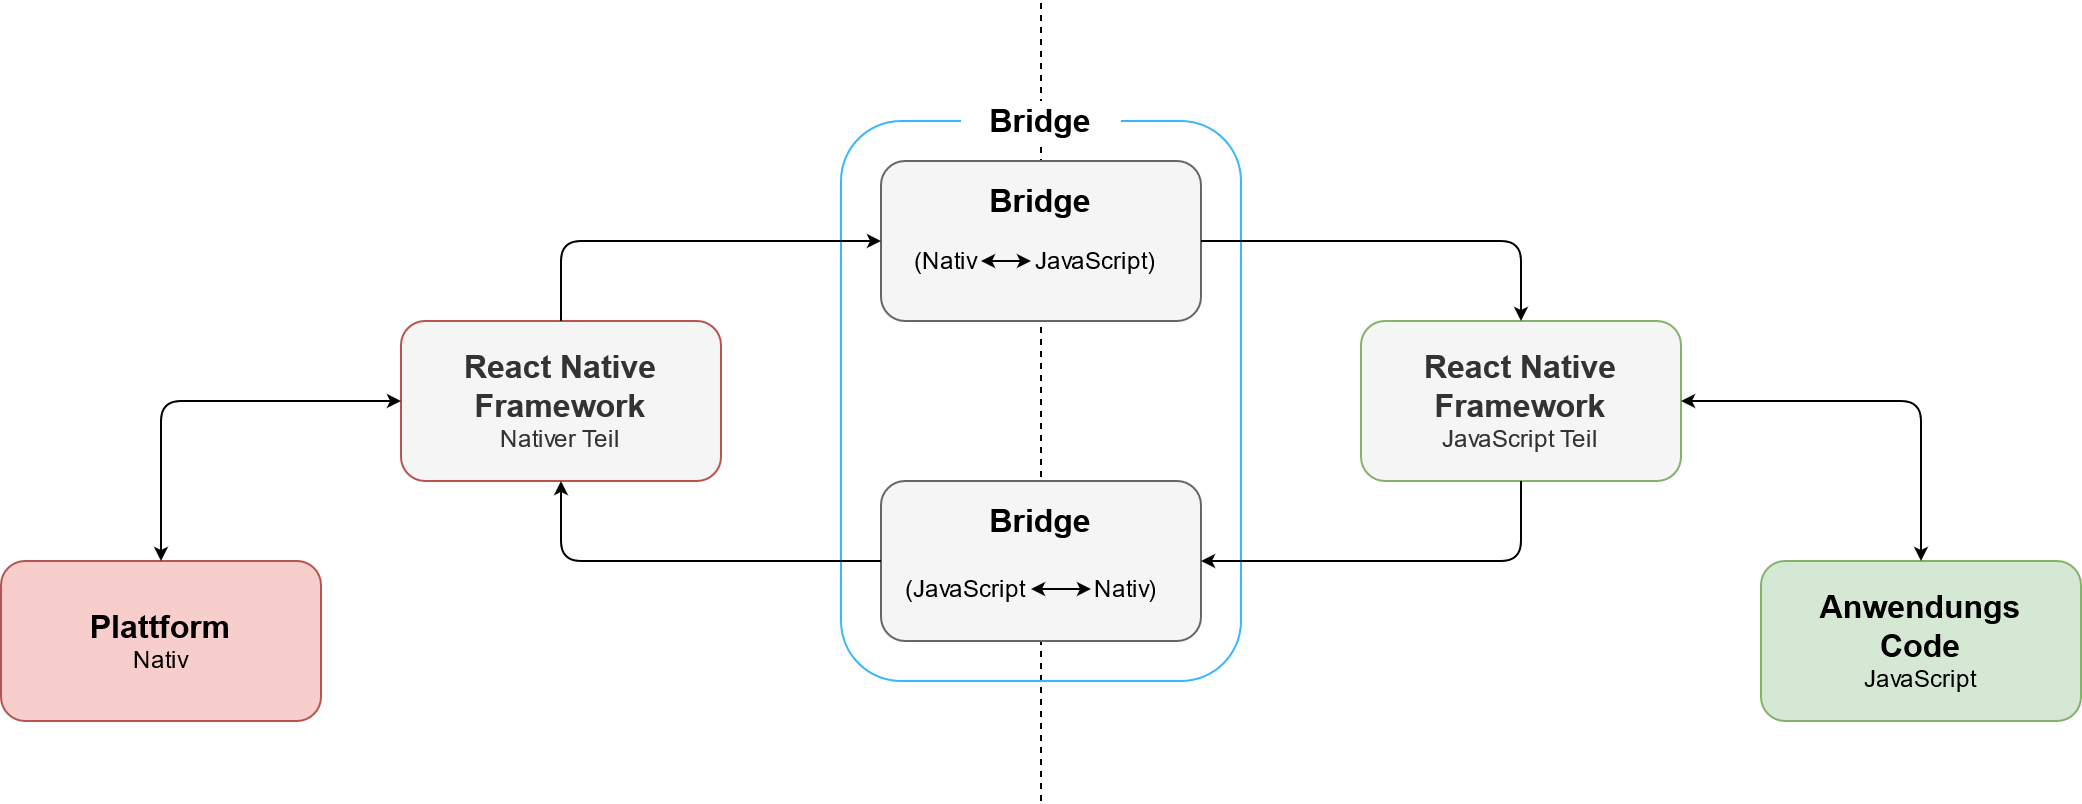
\includegraphics[scale=0.2]{react_bridge}
	\centering
	\caption[Übersicht der Kommunikation des React Frameworks]{Übersicht der Kommunikation zwischen dem Nativen- und JavaScript-Teil des React Frameworks (Anlehnung an \cite{droids_react_intro})}
\end{figure}

Da die gesamte Kommunikation des nativen und des JavaScript Teils über die React Native Bridge laufen, stellt diese einen Engpass dar, welcher zu Performanceeinbußen führt. Vor allem bei Animationen, welche z.B. von der Position des Fingers des Users abhängig sind, muss bis zu 60-mal pro Sekunde über die Bridge kommuniziert werden.

\blockcquote{talKol_react_performance}{
Here lies one of the main keys to understanding React Native performance. Each realm by itself is blazingly fast. The performance bottleneck often occurs when we move from one realm to the other. In order to architect performant React Native apps, we must keep passes over the bridge to a minimum.
}

Um dieses Problem zu beheben, arbeitet das React Native Team derzeit an einer grundlegend neuen Architektur. Diese trägt den Projektnamen Fabric\cite{react_fabric_youtube}.

\newpage
\section{Das Cross-Kompilierende Framework Flutter}

Flutter ist ein von Google entwickeltes Open Source cross-plattform \ac{SDK}, um nativ kompilierte Anwendungen für Web, Desktop und Mobilgeräte ausgehend von einer einzigen Codebasis zu entwickeln. Es wurde 2018 offiziell veröffentlicht und benutzt die ebenfalls von Google entwickelte Programmiersprache Dart\cite{flutter_dev}.\\

Dart ist eine ECMA-Standardisierte Vielzweck-Programmiersprache und wurde ursprünglich als alternative zu JavaScript entwickelt\cite{techcrunch_dart}. Dart ist optional typisiert, somit kennt Dart zwei Laufzeit-Modi: Produktion und Checked. Im Produktionsmodus wählt der Compiler selbstständig einen Typen und ignoriert Typisierungsanweisungen sowie Typfehler, um eine möglichst hohe Effizienz zu gewährleisten. Im Checked-Modus werden Typen strikt beachtet und bei Fehlern Exceptions geworfen. Die dafür notwendige Codeanalyse macht diesen Modus jedoch langsamer. Dart kann je nach Verwendungszweck auf verschiedene Arten kompiliert werden. Dazu gehören für die native Entwicklung \ac{JIT}, \ac{AOT} sowie der dart2js und dartdevc Compiler, welcher aus Dart Code JavaScript für das Web erzeugt\cite{dart_dev}.\\

\begin{figure}[h]
	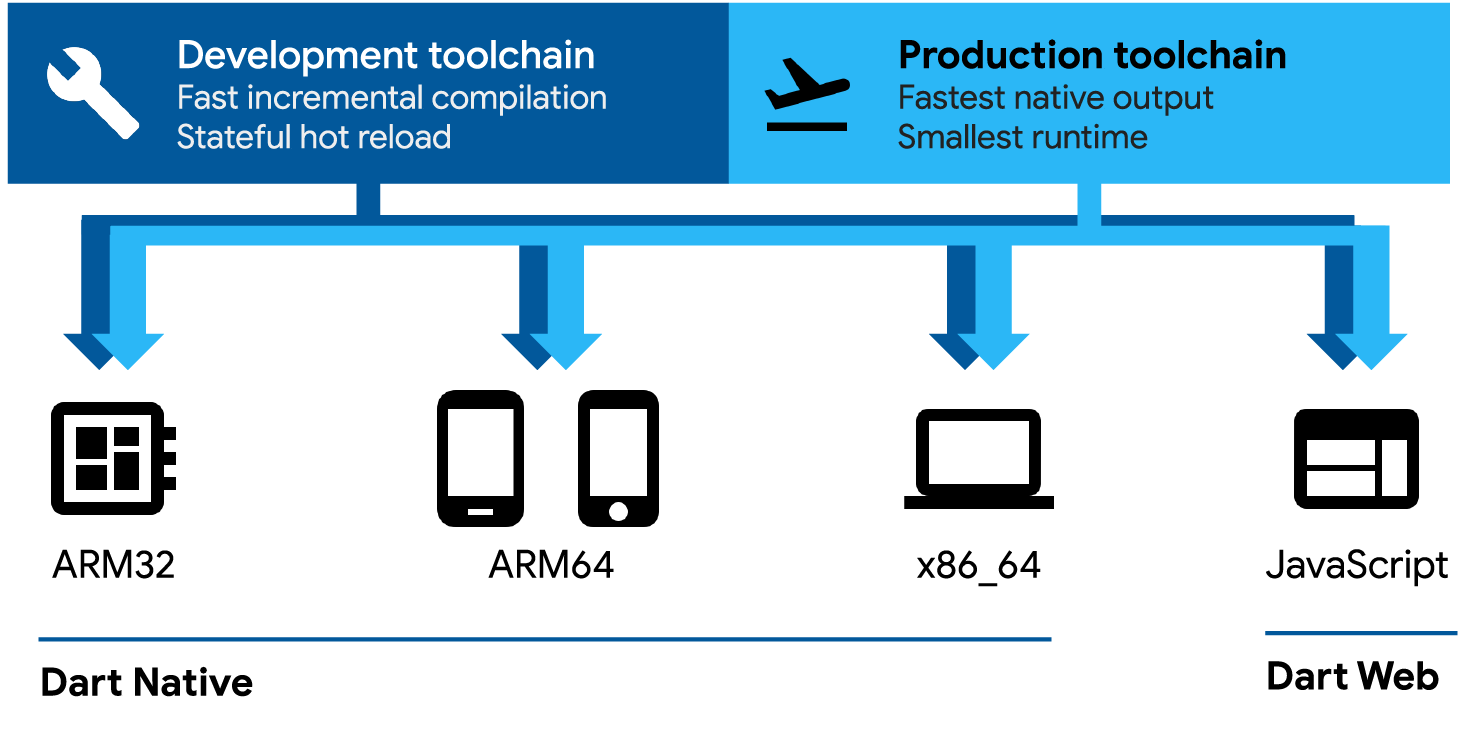
\includegraphics[scale=0.4]{dart_platforms}
	\centering
	\caption[Übersicht der Zielplattformen der Programmiersprache Dart]{Übersicht der Zielplattformen der Programmiersprache Dart \cite{dart_dev}}
\end{figure}


Diese Flexibilität macht Dart einzigartig, in der Hinsicht, dass es die einzige breit verwendete Programmiersprache ist, welche diese Möglichkeiten bietet. Bei der Entwicklung wird meist der \ac{JIT} Ansatz zusammen mit einer Dart \ac{VM} verwendet, da damit der Entwicklungsfluss gefördert wird, da Anpassungen im Quellcode direkt beobachtet werden können. Zum Ausliefern der Anwendung wird diese schließlich \ac{AOT} kompiliert. Der Vorteil von \ac{AOT} kompiliertem Code ist, dass dadurch die Startzeit der Anwendung stark verringert werden kann. Anwendungen, welche den Code zuerst kompilieren müssen, haben aufgrund der notwendigen Codeanalyse und der Kompilation selbst eine längere Startzeit. Es wurde nachgewiesen, dass bei längeren Verzögerungen, User von der Benutzung einer App oder Website absehen, falls die Ladezeit drei Sekunden übersteigt\cite{akamai_abandonment}. Ein weiterer Vorteil des \ac{AOT} Ansatzes ist, dass damit dem Problem der \glqq JavaScript Bridge\grqq\ entgegengewirkt wird. Dieses entsteht durch die Notwendigkeit der Kommunikation zwischen einer dynamischen und somit \ac{JIT} kompilierten Sprache wie JavaScript sowie dem nativen Code der Plattform.\\

Dieses Problem wird durch die \ac{AOT} Kompilation von Dart zwar nicht komplett beseitigt, da dieser ebenfalls über ein Interface mit dem nativen Code kommunizieren muss, jedoch muss kein kompletter Kontextwechsel vollzogen werden. Da Flutter die \ac{UI}-Komponenten selbst mithilfe der mitgelieferten Skia Engine rendert ist die Notwendigkeit häufiger Kommunikation ebenfalls geringer und dadurch ressourcenschonender.
Die Tatsache, dass die \ac{UI}-Komponenten (bei Flutter Widgets genannt) von der Applikation und nicht von der Plattform gerendert werden birgt einige Vorteile. Einerseits sind die UI-Komponenten erweiterbar und anpassbar, andererseits entfällt die Notwendigkeit eines virtuell \ac{DOM}s. Dieser ist bei Frameworks wie React die Grundlage, um die interne Repräsentation des Inhaltes darzustellen und wird bei Veränderungen mit dem tatsächlichen \ac{DOM} verglichen, sodass Unterschiede gebündelt angepasst werden können. Da Flutter die \ac{UI}-Komponenten selber rendert, entfällt die Notwendigkeit und der damit verbundene Aufwand, da der virtuelle \ac{DOM} gleichzeitig den reellen \ac{DOM} darstellt.
Andererseits steigt durch die Tatsache, dass Flutter die UI-Komponenten und den passenden Renderer bereitstellt die Kompatibilität der verschiedenen Betriebssystemversionen. Die Notwendigkeit auf all diesen Versionen testen zu müssen entfällt, da sich die Flutter-Entwickler darum kümmern.
Der Dart Code einer Flutter Anwendung kommuniziert mittels der sogenannten Platform Channels mit dem nativen API der Plattform. Dabei werden keine Abbildungen von Dart Code zu nativen \ac{API}-Aufrufen verwendet, sondern bidirektionale Nachrichten, welche asynchron verarbeitet werden und mithilfe von Callbacks dem Aufrufer ihr Ergebnis mitteilen. Dadurch entfällt der Engpass der zentralen Bridge.\\

\begin{figure}[h]
	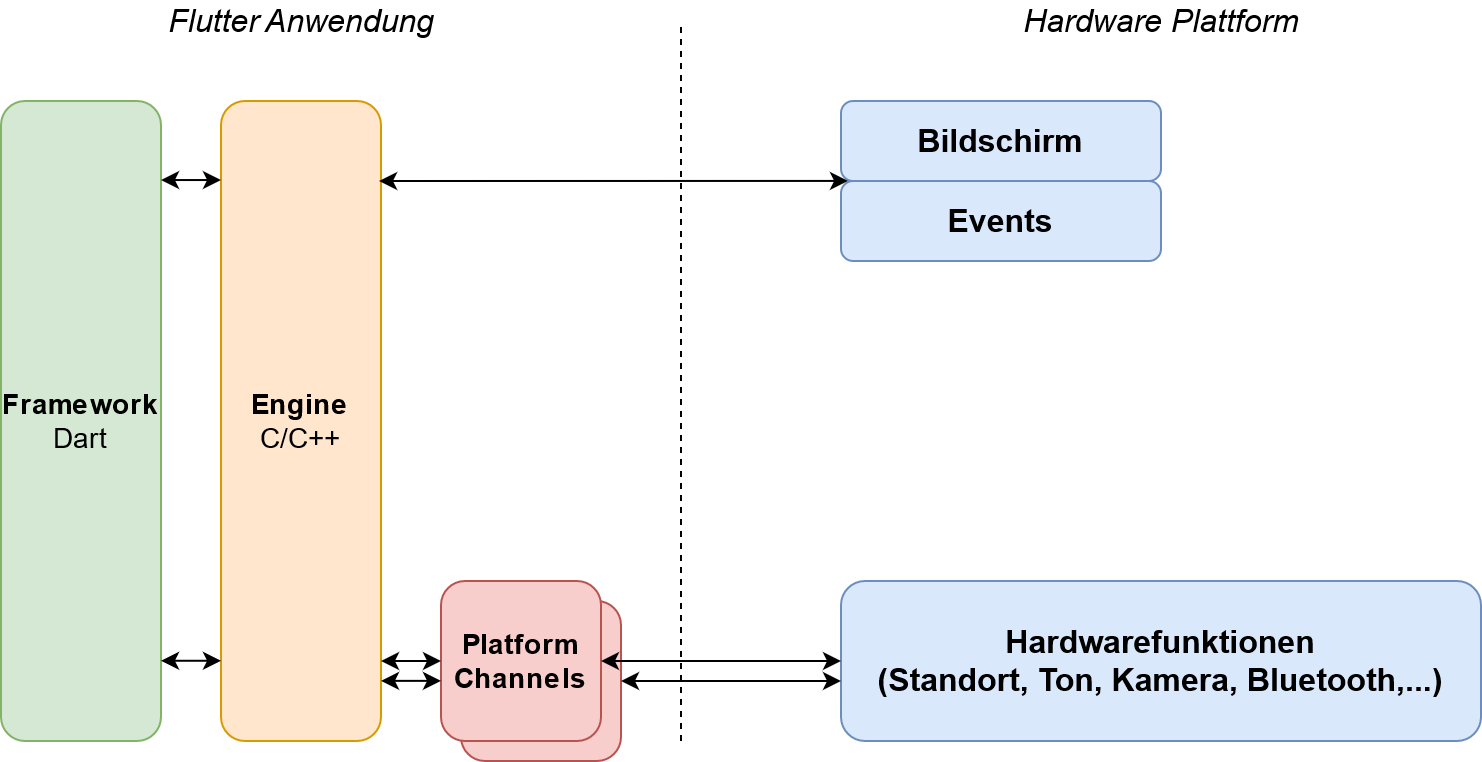
\includegraphics[scale=0.2]{flutter_architecture}
	\centering
	\caption{Vereinfachtes Schema einer Flutter Anwendung}
\end{figure}

Im Allgemeinen ähnelt das Flutter Framework einer Game Engine. Da Flutter Anwendungen aus dem Framework selbst (Dart), einer performanten Rendering Engine (C/C++) und einem plattformspezifischen Teil bestehen, welcher den Einstiegspunkt der Anwendung bildet und sich um die Kommunikation mit dem Betriebssystem kümmert.



	\chapter{Fazit}

Die Entwicklung einer Anwendung mithilfe eines cross-plattform Frameworks verringert den Entwicklungsaufwand und die dafür notwendige Zeit. Dies führt zu schnelleren Ergebnissen, da die Anwendung nur auf einer Codebasis aufbaut. Jedoch existiert einer Vielzahl an verschiedenen Entwicklungsansätzen, welche alle bestimmte Vor- und Nachteile bieten. Dazu gehören (Progressive) Web-Apps, hybride Apps, Apps mit eigener Laufzeitumgebung, cross-kompilierte sowie generierte Apps.\\

Allgemein lässt sich feststellen, dass native Apps die meisten Features bieten, dies jedoch  auf Kosten der Notwendigkeit zwei komplett eigenständige Anwendungen entwickeln zu müssen. Auf der anderen Seite des Spektrums befinden sich Web-Applikationen, welche einfacher zu entwickeln und pflegen sind, meist jedoch nicht die benötigen Features bereitstellen. Diese Lücke versuchen \ac{PWA}s zu füllen, indem diese einige native Funktionalitäten bereitstellen und somit die größten Nachteile der Web-Applikationen aufheben. Hybride App Frameworks versuchen die Vorteile der Entwicklung mit Web-Technologie sowie den Zugang zu Hardware-Features für die Erstellung von Apps, welche über den App-Store verteilt werden können, zugänglich zu machen. Diese haben jedoch den Nachteil, dass damit der native \glqq Look and Feel\grqq\ einer nativen App nicht trivial repliziert werden kann. Auf einer eigenen Laufzeitumgebung basierende Apps versuchen diesen Nachteil zu umgehen, in dem native \ac{UI}-Komponenten verwendet werden, welche mit JavaScript definiert werden können. Einen neuen Weg versucht das Flutter Framwork zu gehen. Dieses cross-kompilierende Framework verwaltet die Darstellung und Rendering der \ac{UI}-Komponenten selbst und versucht somit die Performance-Probleme der Framworks mit eigenständiger Laufzeitumgebung zu beheben. Der aktuelle Trend spricht derzeit für diesen Game-Engine-ähnlichen Ansatz, jedoch bleibt abzuwarten, ob sich dieser Trend fortsetzt, da die Entwicklung sich noch am Anfang befindet.\\

\newpage

Welches Framework sollte denn nun für das nächste Projekt verwendet werden?
Diese Frage ist stark einzelfallabhängig und es gibt, wie so häufig, keine eindeutige Antwort. Jedoch möchte ich trotzdem einige grundsätzliche Fragen formulieren, welche bei der Evaluation solcher Frameworks beantwortet werden können, um die Auswahl zu vereinfachen.
Zunächst wäre es sinnvoll folgende Fragen bezüglich der Anwendung und der Zielgruppe zu beantworten.\\


\begin{multicols}{2}
	\begin{itemize}
		\vspace{-2mm}
		\setlength\itemsep{0mm}
		\item Welches Problem wird mit der Anwendung für wen gelöst?
		\item Welche Technik ist die Zielgruppe vertraut?
		\item Mit welchen Entwicklungsansätzen, Sprachen und Frameworks sind die Entwickler vertraut?
		\item Wie soll die Anwendung verteilt werden? (App-/Playstore oder Browser)
		\item Wie performant soll die Anwendung sein?
		\item Wie viele und welche plattformspezifische Features sollen verwendet werden?
		\item Ist eine Internetverbindung am Einsatzort verfügbar?
		\item Müssen spezifische Zertifizierungen wie z.B. im Gesundheits- und Finanzsektor erfüllt werden?
	\end{itemize}
\end{multicols}

Erst nachdem die vorangestellten Fragen beantwortet wurden, sollten die verschiedenen Vor- und Nachteile der verschiedenen Entwicklungsansätzen gegeneinander aufgewogen und verglichen werden.\\

Aufgrund der in der Arbeit genannten Punkte ist es für ein Team, welches keine ausgeprägten Kenntnisse mit Web-Technologien besitzt, meistens besser Flutter zu verwenden. Falls im Entwicklerteam bereits Web-Kenntnisse mit React vorhanden sind, ist React Native eine sinnvolle Wahl. Ansonsten bietet Ionic eine flexible Alternative, da dort verschiedene Front-End-Frameworks verwendet werden können.


	%%%Ab hier werden die einzelnen Kapitel als extra .tex Dateien angehängt
	%%%Die Kapitel brauchen dabei keine Formatierungen, nur Überschriften etc.
	%%%Alle .tex in einem Ordner%%%
	%\input{}
	\printbibliography[heading=bibintoc,title={Literaturverzeichnis}]
	
	%\clearpage
	
	%\chapter{Anhang}
	
	
	
\end{document}